% !TeX encoding = UTF-8
\documentclass[12pt]{article}

\usepackage{setspace}
\usepackage{CJKutf8}
\usepackage{enumitem}
\usepackage{array}
\usepackage{multirow}
\usepackage{amsmath}
\usepackage{graphicx}
\usepackage{subcaption}
\usepackage{setspace}
\usepackage{wallpaper}
\usepackage{adjustbox}
\usepackage{afterpage}
\usepackage{lscape}
\usepackage{mathptmx}
\usepackage{titlesec}
\usepackage{float}
\floatstyle{plaintop}
\restylefloat{table}
\floatstyle{plain}
\restylefloat{figure}
\usepackage[labelfont=bf,textfont=bf]{caption}
\usepackage[hyphens]{url}
\usepackage[margin=2.8cm]{geometry}
% \addtolength{\wpXoffset}{+9.26cm}
% \addtolength{\wpYoffset}{-12.5cm}
% \usepackage[backend=ieee]{biblatex}
% \usepackage{biblatex}
\usepackage[numbers,sort]{natbib}
\setcitestyle{square,citesep={],[}}
% \bibliography{main}
\usepackage{booktabs}
\usepackage{siunitx}
\sisetup{
  round-mode = places,
  round-precision = 2,
}
\usepackage{listings}
\usepackage{color}
\usepackage{hyperref}
\hypersetup{
    colorlinks,
    citecolor=black,
    filecolor=black,
    linkcolor=black,
    urlcolor=black
}
\makeatletter

\newif\if@mainmatter \@mainmattertrue

\newcommand\frontmatter{%
    \cleardoublepage
  \@mainmatterfalse
  \pagenumbering{roman}}
\newcommand\mainmatter{%
    \cleardoublepage
  \@mainmattertrue
  \pagenumbering{arabic}}
\makeatother

\renewcommand\lstlistingname{Figure}
\renewcommand\lstlistlistingname{Figures}

\DeclareCaptionLabelFormat{tablel}{#1 #2}
\captionsetup[table]{labelsep=period,font={stretch=1.77}}
\captionsetup[figure]{labelsep=period,font={stretch=1.77}}

\lstset{
  language=XML,
  morekeywords={encoding,
  xs:schema,xs:element,xs:complexType,xs:sequence,xs:attribute}
}

\title{Recognizing Chinese Textual Entailment by Deep Learning}
\author{
  Wei-Ting Chen\\
  National Taiwan Ocean University\\
  \texttt{10757025@mail.ntou.edu.tw}\\
  \\
  Chuan-Jie Lin\\
  Nation Taiwan Ocean University\\
  \texttt{cjlin@mail.ntou.edu.tw}\\
}

\titleclass{\subsubsubsection}{straight}[\subsection]

\newcounter{subsubsubsection}[subsubsection]
\renewcommand\thesubsubsubsection{\thesubsubsection.\arabic{subsubsubsection}}
\renewcommand\theparagraph{\thesubsubsubsection.\arabic{paragraph}}

\titleformat{\subsubsubsection}
  {\normalfont\normalsize\bfseries\itshape}{\thesubsubsubsection}{1em}{}
\titlespacing*{\subsubsubsection}
{0pt}{3.25ex plus 1ex minus .2ex}{1.5ex plus .2ex}

\makeatletter
\renewcommand\paragraph{\@startsection{paragraph}{5}{\z@}%
  {3.25ex \@plus1ex \@minus.2ex}%
  {-1em}%
  {\normalfont\normalsize\bfseries}}
\renewcommand\subparagraph{\@startsection{subparagraph}{6}{\parindent}%
  {3.25ex \@plus1ex \@minus .2ex}%
  {-1em}%
  {\normalfont\normalsize\bfseries}}
\def\toclevel@subsubsubsection{4}
\def\toclevel@paragraph{5}
\def\toclevel@paragraph{6}
\def\l@subsubsubsection{\@dottedtocline{4}{7em}{4em}}
\def\l@paragraph{\@dottedtocline{5}{10em}{5em}}
\def\l@subparagraph{\@dottedtocline{6}{14em}{6em}}
\makeatother

\setcounter{secnumdepth}{4}
\setcounter{tocdepth}{4}

\begin{document}
\begin{CJK*}{UTF8}{bkai}

\begin{titlepage}
  \centering
  {\Huge 國立臺灣海洋大學\par}
  \vspace{1cm}
  {\huge 資訊工程學系\par}
  \vspace{1cm}
  {\huge 碩士學位論文\par}
  \vspace{2cm}
  {\LARGE 指導教授:林川傑\ (Lin, Chuan-Jie) 博士\par}
  \vfill
  {\LARGE 以深度學習辨識中文文本蘊涵關係\par}
  {\LARGE Recognizing Chinese Textual Entailment by Deep Learning\par}
  \vfill
  {\LARGE 研究生:陳威廷\ \bigg(
    \begin{tabular}{c}
      Chen, Wei-Ting \\
      M10757025
    \end{tabular}
    \bigg) 撰}
    \vfill
    {\LARGE 中華民國\ 110 年\ 07 月}
\end{titlepage}

\newpage

\CenterWallPaper{0.7}{ntou.png}

\begin{titlepage}
  \centering
  {\LARGE 以深度學習辨識中文文本蘊涵關係\par}
  \vfill
  {\Large Recognizing Chinese Textual Entailment by Deep Learning\par}
  \vfill
  {
    \Large
    \begin{minipage}{2in}
      研究生:陳威廷 \\
      指導教授:林川傑
    \end{minipage}
    \hfill
    \begin{minipage}{2.4in}
      Student: Chen, Wei-Ting \\
      Advisor: Lin, Chuan-Jie
    \end{minipage}
    \par
  }
  \vfill
  {\LARGE 國立臺灣海洋大學\par}
  {\LARGE 資訊工程學系\par}
  {\LARGE 碩士學位論文\par}
  \vfill
  {
    \LARGE
    A Thesis \\
    Submitted to Computer Science and Engineering \\
    Electrical Engineering and Computer Science \\
    National Taiwan Ocean University \\
    In Partial Fulfillment of the Requirements \\
    for the Degree of \\
    Master of Science \\
    in \\
    Computer Science and Engineering \\
    March, 2021 \\ \vspace{0.5cm}
    Keelung, Taiwan, Republic of China
  }
  \vfill
  {\LARGE 中華民國\ 110 年\ 07 月}
\end{titlepage}
\ClearWallPaper
\pagenumbering{gobble}
\titleformat{\section}{\clearpage\centering\bfseries\LARGE}{Chapter \thesection.}{0.5em}{}
\newpage

\begin{spacing}{1.77}

\frontmatter
\phantomsection
\addcontentsline{toc}{section}{摘要}
\section*{摘要}
\paragraph{}
本研究為文意蘊含系統,主要使用了深度學習的方法並透過額外的資料集進行訓練。我們在探討了各種不同的特徵、分類器以及訓練手法後設計而成。

\paragraph{}
在特徵方面,使用了包含適合機器學習的文句特徵以及適合深度學習的字詞特徵。在分類器方面,除了基本的\ SVM 以外,還有\ MLP、RNN 以及近年來在\ NLP 領域很受歡迎的\ Transformers BERT。在訓練手法方面,我們使用了額外資料集進行了跨語言訓練,並使用規則式與\ GPT-2 模型產生虛擬訓練資料來改善系統效能。

\paragraph{}
最終實驗結果顯示,透過\ MNLI 資料集對\ BERT 進行跨語言訓練,分別在\ RITE-VAL 與\ RITE2 測試資料集上達到\ F1-Score 為\ 0.5561\ /\ 0.7107 的效能,其結果巨幅超越\ NTCIR 官方所宣佈的系統。

\newpage
\phantomsection
\addcontentsline{toc}{section}{Abstract}
\section*{Abstract}
\paragraph{}
% 本研究為文意蘊含系統,主要使用了深度學習的方法並透過額外的資料集進行訓練。我們在探討了各種不同的特徵、分類器以及訓練手法後設計而成。
This thesis propose a textual entailment recognizing system by deep learning using transformers training through additional datasets. We design this system after discussing various feature approaches, classifiers, and training techniques.

\paragraph{}
% 在特徵方面,使用了包含適合機器學習的 Sentence-based features 以及適合深度學習的 word-based sequence features。在分類器方面,除了基本的 SVM 以外,還有 MLP、RNN 以及近年來在 NLP 領域很受歡迎的 Transformers BERT。在訓練手法方面,我們使用了額外資料集進行了跨語言領域的訓練,並使用 GPT-2 模型產生虛擬訓練資料來改善系統效能。
In the feature approaches, we use sentence-based features which are suitable for machine learning, and word-based sequence features which are suitable for deep learning. In the classifiers, besides basic machine learning classifier SVM, we also use the feedforward neural network, the recurrent neural network, and the transformers BERT, which is popular in the natural language process domain recent years. In the training techniques, we use additional datasets to do the cross-lingual training and use the GPT-2 model to generate the pseudo training data to improve the performance of the system.

\paragraph{}
% 最終實驗結果顯示,透過 MNLI 資料集對 BERT 進行跨語言的訓練分別在 RITE-VAL 與 RITE2 測試資料集上的 F1-Score 效能來到 0.5561/0.7107,其效能巨幅超越 NTCIR 官方所宣佈的系統。
The experiment results show that the cross-lingual training for BERT through MNLI has achieved an F1-measure of 0.5561 and 0.7107 to RITE-VAL and RITE2, this system greatly outperformed the best system in the NTCIR RITE-VAL and RITE2 Traditional Chinese subtask.

\paragraph{Keywords} natural language process, natural language inference, recognizing textual entailment, machine learning, deep learning, transformers.

\newpage

% \section*{Acknowledgements}
% 誌謝
% \newpage
\end{spacing}

\begin{spacing}{1.77}
\phantomsection
\addcontentsline{toc}{section}{Contents}
\tableofcontents

\newpage
\phantomsection
\addcontentsline{toc}{section}{List of Figures}
\listoffigures
\newpage
\phantomsection
\addcontentsline{toc}{section}{List of Tables}
\listoftables
\end{spacing}
\newpage

\pagenumbering{arabic}

\newcommand{\PreserveBackslash}[1]{\let\temp=\\#1\let\\=\temp}
\newcolumntype{C}[1]{>{\PreserveBackslash\centering}p{#1}}
\newcolumntype{R}[1]{>{\PreserveBackslash\raggedleft}p{#1}}
\newcolumntype{L}[1]{>{\PreserveBackslash\raggedright}p{#1}}

\begin{spacing}{1.77}
\section{Introduction} \label{section:introduction}

\subsection{Motivation}
\paragraph{}
% NLI 任務在定義上並不複雜,給定一句 Premise 和一句 Hypothesis,並辨識這兩句話是否存在蘊含關係。一個文意蘊含任務的分類有很多種類型,最簡單的分法就是「有蘊含」與「沒有蘊含」,而「沒有蘊含」的部份可以進一步的分成「互斥」與「獨立」,「有蘊含」的部份也可以進一步的分成「正向蘊含」與「雙向蘊含」。去判別兩句話之間是否存在蘊含關係,這個任務的難度會因為涉及的語言現象而產生很高的複雜度
The definition of the recognizing textual entailment (RTE), or natural language inference (NLI), is the entailment-related relation between two sentences. That is, given that the state described in the first sentence is true, the state described in the second sentence will be true or not.

\paragraph{}
There are many ways to define categories of textual entailment relations. The simplest one is binary decision, i.e. ``entailment'' and ``not entailment''. The category of ``not entailment'' can be further divided into ``contradiction'' and ``independence''. The category of ``entailment'' can be further divided into ``forward entailment'' and ``bidirectional entailment''. The determination of the relation of the two sentences may be difficult if the linguistic phenomena of the sentences are complicated.

\paragraph{}
% 模型是否能夠精準判別此蘊含關係,是衡量此模型的自然語言理解能力很重要的指標。在許多自然語言的應用中,例如:問答系統、文件摘要、資訊擷取與機器翻譯等,若是能提高模型的語言理解能力,將會是相當有幫助的事情。
Recognizing textual entailment is an important indicator to measure the natural language understanding ability of NLP systems. Increasing the NLU ability will be helpful in many NLP applications, such as question answering, summarization, information extraction, and machine translation. Deep learning had achieved huge success on the RTE tasks, but most of them used large-scale datasets and expensive models.

\paragraph{}
There have been many Chinese RTE datasets, including RITE, CNLI, and OCNLI. Among them, CNLI and OCNLI seem easier, since the performances of the state-of-the-art systems are above 0.8 in accuracy. However, the performances of RITE are only 0.4 to 0.5 in f1-measure. We think RITE datasets are more difficult because they are small-scale datasets and contain abundant linguistic phenomena.

\paragraph{}
% 近年來深度學習在 NLI 任務上取得了巨大的成功,但多數的成果都是僅限於大型英文資料集。本論文將會以繁體中文的 NLI 資料集 - RITE 為主要目標,將這份成功帶到這份相對小型的繁體中文資料集上面。
This thesis focuses on improving deep learning systems evaluated on RITE datasets. We try several approaches including integrating machine learning features, word alignment, cross-lingual training, and generating pseudo training data.

\subsection{Related Work} \label{sec:related_work}
\subsubsection{Textual Entailment Datasets}
\paragraph{}
In English NLI datasets, the Stanford Natural Language Inference (SNLI)\footnote{https://nlp.stanford.edu/projects/snli/} \cite{snli:emnlp2015} is a well-known corpus of the NLI datasets, which is a collection of 570k human-written English sentence pairs.

\paragraph{}
GLUE benchmark\footnote{https://gluebenchmark.com/} collected many NLI datasets as their NLP task benchmark, including RTE, MNLI, QNLI, WNLI. The Recognizing Textual Entailment (RTE) datasets come from a series of annual textual entailment challenges. RTE1 \cite{dagan2006pascal}, RTE2 \cite{bar2006second}, and RTE3 \cite{giampiccolo2007third} are provided by PASCAL\footnote{http://pascallin.ecs.soton.ac.uk/}, RTE4, RTE5 \cite{bentivogli2009fifth}, RTE6, and RTE7 are provided by NIST\footnote{https://www.nist.gov/}.

\paragraph{}
The Multi-Genre Natural Language Inference (MultiNLI, or MNLI)\footnote{https://cims.nyu.edu/~sbowman/multinli/} \cite{N18-1101} is a crowd-sourced collection of 433k sentence pairs collected from a wide range of genres. Question-Answering NLI (QNLI) \cite{wang2019glue} dataset is an NLI dataset converting from the Stanford Question Answering Dataset v1.1 (SQuAD) \cite{rajpurkar2016squad}.

\paragraph{}
The Winograd NLI dataset (WNLI) is also an augmented dataset, coming from a reading comprehension task called The Winograd Schema Challenge \cite{levesque2011winograd}. The Cross-Lingual Natural Language Inference (XNLI)\footnote{https://github.com/facebookresearch/XNLI} has 7.5k sentence pairs and has been translated into 14 languages, including English and Simplified Chinese, which results in 112.5k annotated pairs.

\paragraph{}
In Chinese NLI datasets, Chinese Natural Language Inference (CNLI)\footnote{https://github.com/blcunlp/CNLI} is a Simplified Chinese dataset from a share task of the Seventeenth China National Conference on Computational Linguistics (CCL 2018) which has 90k sentence pairs. Original Chinese Natural Language Inference (OCNLI) is a NLI dataset with 50k sentence pairs, and it is a part of CLUE benchmark\footnote{https://www.cluebenchmarks.com/}.

\paragraph{}
NTCIR\footnote{https://research.nii.ac.jp/ntcir/} held several RTE tasks, they are two RITE tasks in NTCIR-9 \cite{ntcir9rite1} and NTCIR-10 \cite{ntcir10rite2}, and RITE-VAL task in NTCIR-11 \cite{ntcir11rite-val}. Several RITE datasets are constructed in Japanese, Traditional Chinese, and Simplified Chinese.

% In NTCIR-9 \cite{ntcir9rite1}, NTCIR-10 \cite{ntcir10rite2}, and NTCIR-11 \cite{ntcir11rite-val}, they proposed the RITE datasets, which have Japanese, Traditional Chinese, and Simplified Chinese subtasks.
% Related NLI dataset, RTE \cite{dagan2006pascal} \cite{bar2006second} \cite{giampiccolo2007third}, SNLI, MNLI, QNLI \cite{wang2019glue}, CNLI, OCNLI, RITE.
\subsubsection{Machine Learning Based Systems}
% 與我們同實驗室的 Tu 等人在 RITE1 與 RITE2 的 BC Task 上取得了 71.05% 與 66.62% 的 F-scores,而在 MC Task 上則達到 53.27% 與 48.39% 的 F-scores. 這些成果都比 NTCIR-9 與 NTCIR-10 的參賽系統都來得好。之後的 Liu 等人則擴展了上個方法,將之應用在 RITE-VAL 上,其效能也同樣勝過 NTCIR-11 的參賽系統。
\paragraph{}
Zanzotto and Moschitti \cite{zanzotto_moschitti_2006} conducted the experiments with the datasets of the RTE 2005 challenge by using cross-pair similarities and achieved 63.88\% in accuracy. Wang and Neumann \cite{wang_neumann_2007} had achieved an accuracy of 66.9\% on the RTE-3 dataset by using sentence similarity based on dependency tree skeletons. Dinu and Wang \cite{dinu_wang_2009} focused on the inference rules and try to find the improvement and achieved 61.75\% in accuracy with RTE-3 dataset.

\paragraph{}
Shih \emph{et al}. \cite{Shih2013IASLRS} developed a two-stage knowledge-based textual inference recognition system and achieved the F-scores of 0.6714 and 0.4632 for NTCIR-10 RITE2 Traditional Chinese BC and MC subtasks. We \emph{et al}. \cite{WuHLLCK14} detected special cases of the sentence pair and used several SVM classifiers to do classification. This system achieved F-scores of 0.5672 and 0.4054 for NTCIR-11 RITE-VAL Traditional Chinese SVBC and SVMC subtasks.

% \paragraph{}
% Su and Zheng \cite{su_zheng_2011} achieved the best precision of 55.9\% on NTCIR-9 RITE by using C4.5 decision tree base on the lexical and semantic features. Wang \emph{et al}. \cite{wang-etal-2013-labeled} achieved the best accuracy of 74.65\% on NTCIR-10 RITE2 Simplified Chinese BC subtask by labeled alignment, but they did not evaluate their system on the MC subtask dataset.

\paragraph{}
Lin and Tu \cite{tu_2014_paper} combined a rule-based classifier and a SVM classifier, which achieved the F-scores of 71.05\% and 66.62\% to the BC task of RITE1 and RITE2, and the F-scores of 53.27\% and 48.39\% to the MC task. This system outperformed the best systems of NTCIR-9 and NTCIR-10. Liu \emph{et al}. \cite{liu_2016_paper} extended this system and applied on RITE-VAL which achieved 48.61\% in F-scores. This system outperformed the best systems of NTCIR-11 RITE-VAL.

\subsubsection{Neural Network}
% System/MNLI/RTE
% BERT/86.7/70.1
% Albert/91.3/89.2
% RoBERTa/90.8/88.2
% SemBERT/87.6/84.5
% MTDNN/86.7/81.4
% XLNET/90.9/88.5
% T5/92.2/92.8
% ERNIE/84.0/68.8
% DeBERTa/91.1/88.3

% === 新增的部份 ===
\paragraph{}
When representing a sentence by a single vector, MLP is a common choice to build a classifier. Multilayer perceptron (MLP), also known as feedforward neural network, is the simplest form of artificial neural network. The information of the perceptron only passes through one direction, the neurons in the same layer do not communicate with each other.

\paragraph{}
To process variable-length of sentences, we use the recurrent neural network. Recurrent neural network (RNN) is a type of neural network layer constructed by the neurons with internal state. The neurons inside a recurrent neural network layer will communicate with each other to affect the internal state and produce the effect of memory.

% Therefore, the recurrent neural network can process a variable-length sequence of inputs, make it suitable for natural language processing such as RTE tasks.

\paragraph{}
The recurrent neural networks have multiple variants. We will compare three basic types of recurrent neural networks: vanilla recurrent neural network, long short-term memory (LSTM) \cite{hochreiter1997lstm}, and gated recurrent unit (GRU) \cite{cho2014gru}.

\paragraph{}
Vaswani \emph{et al}. \cite{vaswani2017attention} created the attention mechanism that mimicked cognitive attention. When delivering information between layers, the important parts will be enhanced and fade out the unimportant parts. Which parts are more important depends on the training data and learned by gradient backpropagation. Using the attention mechanism in the recognizing textual entailment task will make the model more concentrated on the key information.

% Vaswani \emph{et al}. \cite{vaswani2017attention} created the attention mechanism that mimicked cognitive attention, and proposed the architecture of transformers. This model achieved a great performance on machine translation task.

\paragraph{}
The structure of transformer \cite{vaswani2017attention} uses multi-head attention to build the encoder-decoder model, which uses to solve the machine translation tasks. Devlin \emph{et al}. \cite{devlin2018bert} proposed BERT\footnote{https://github.com/google-research/bert} that extended the transformers onto many NLU tasks and achieved an accuracy of 86.7\% on MNLI and an accuracy of 70.1\% on RTE.

% === 新增的部份 ===

\paragraph{}
RoBERTa \cite{liu2019roberta} optimized the pre-training approach of BERT and achieved an accuracy of 90.8\% on MNLI and an accuracy of 88.2\% on RTE. ALBERT\footnote{https://github.com/google-research/albert} \cite{lan2020albert} reduced the parameters of BERT and achieved an accuracy of 91.3\% on MNLI and an accuracy of 89.2\% on RTE.

\paragraph{}
SemBERT\footnote{https://github.com/cooelf/SemBERT} \cite{zhang2020sembert} incorporated the contextual semantics to improve the results on reading comprehension task, and achieved an accuracy of 87.6\% on MNLI and an accuracy of 84.5\% on RTE. Liu \emph{et al}. \cite{liu2019mtdnn} proposed MT-DNN\footnote{https://github.com/microsoft/MT-DNN} which made the language representation more general to adapt to new tasks and domains, and achieved an accuracy of 86.7\% on MNLI and an accuracy of 81.4\% on RTE.

\paragraph{}
XLNET\footnote{https://github.com/zihangdai/xlnet} \cite{yang2020xlnet} is a generalized autoregressive pre-training method that overcomes the limitations of BERT. It achieved an accuracy of 90.9\% on MNLI and an accuracy of 88.5\% on RTE. T5\footnote{https://github.com/google-research/text-to-text-transfer-transformer} \cite{raffel2020t5} used a unified text-to-text transformer to explore the limits of transfer learning, and achieved an accuracy of 92.2\% on MNLI and an accuracy of 92.8\% on RTE.

\paragraph{}
ERNIE\footnote{https://github.com/thunlp/ERNIE} \cite{zhang2019ernie} is an enhanced language representation model which takes full advantage of lexical, syntactic, and knowledge information of the knowledge graphs. It achieved an accuracy of 84.0\% on MNLI and an accuracy of 68.8\% on RTE. DeBERTa\footnote{https://github.com/microsoft/DeBERTa} \cite{he2021deberta} uses the disentangled attention mechanism and the enhanced mask decoder to improve the efficiency of model pre-training and the model performance. It achieved an accuracy of 91.1\% on MNLI and an accuracy of 88.3\% on RTE.

\paragraph{}
Most of these models are only available in English. Since our targets are Chinese datasets, we only use BERT which is available both in Chinese and multilingual versions.

% \subsubsection{Feedforward Neural Network}
% \label{section:simple_dnn}
% \paragraph{}
% 神經網路的蓬勃發展使機器學習在各領域上都獲得了不小幅度的進展,
% Dense Neural Network, Recurrent Neural Network (LSTM, GRU), Attention Mechanism, Transformers
% MLP 模型是只使用了一層 Dense Layer 的模型,透過 Tensorflow 套件建立而成。這個模型架構設計很單純,只用來接收 ML Features。
% feed forward 也稱為 MLP,是最簡單的 ANN 形式,其資訊只會朝著單一方向傳遞,而相同層之間的 Neurons 並不互相傳遞資訊。在本論文中使用的 MLP 模型,是只包含了輸入層、隱藏層、輸入層等基本的 MLP 模型,主要以 Sentence-based features 做為輸入的分類器。
% Multilayer perceptron (MLP), also known as feedforward neural network, is the simplest form of artificial neural network. The information of the perceptron only passes through one direction, the neurons in one layer do not communicate with each other. Multilayer perceptron using in our experiments is the model that only contains an input layer, a hidden layer, and an output layer. This model is use to receive sentence-based features.
% MLP is a neural network only contains one dense layer as a hidden layer, building by Tensorflow API. This model architecture is pretty simple, only use to receive machine learning features

% \subsubsection{Recurrent Neural Network}
% \label{section:rnn}
% \paragraph{}
% Recurrent neural network 是由含有 internal state 的 neurons 所組成的 neural network layer,其特色在於 neuron 內的 internal state 可以建立記憶的效果,使得神經網路可以接收任意長度的輸入,是很適合在 NLP 領域使用的神經網路,因為 NLP 領域經常在處理文本長度不一的任務。
% A recurrent neural network (RNN), is a type of neural network layer constructed by the neurons with internal state. Different from feedforward neural network, the neurons inside a recurrent neural network layer will communicate with each other to affect the internal state and produce the effect of memory. Therefore, the recurrent neural network can process a variable-length sequence of inputs, make it suitable for natural language processing since we usually deal with the text of different lengths. The recurrent neural networks have multiple variants. We will compare three basic types of recurrent neural networks: vanilla recurrent neural network, long short-term memory (LSTM), and gated recurrent unit (GRU).
%
% The RNN-Attention Model (RA Model) is a combination of several different numbers and orders of RNN layers and attention layers.

% Vaswani \emph{et al}. 提到了 Attention mechanism,用來模仿人類注意力的技巧,在傳遞資訊時,強化重要的部份的訊號,減弱不重要的部份,並透過反向傳播梯度來學習何為重要的資訊。在 NLI 任務中使用這個機制,可以讓模型更專注於影響蘊含關係的關鍵資訊上。在實驗中,我們透過不同組合與順序的 RNN 與 Attention 來建構以 Word-based sequence input 為輸入的模型。

% \paragraph{}
% The attention mechanism is described in Vaswani \emph{et al}. \cite{vaswani2017attention}, it is a technique that mimics cognitive attention. When delivering information between layers, the important parts will be enhanced and fade out the unimportant parts. Which parts are more important depends on the training data and learned by gradient backpropagation. Using the attention mechanism in the recognizing textual entailment task will make the model more concentrated on the key information. In our experiments, we construct the model using word-based sequence inputs by the different combinations and orders of the recurrent neural network layer and attention layer.

% \subsubsection{BERT}
% \paragraph{}
% The structure of transformer \cite{vaswani2017attention} uses multi-head attention to build the encoder-decoder model, which uses to solve the machine translation tasks. On the other hand, BERT \cite{devlin2018bert} also used the transformer architecture to achieve excellent performance on several natural language processing tasks, including MNLI, QNLI, and RTE which are contained in GLUE benchmark. The source code of BERT are available on GitHub\footnote{https://github.com/google-research/bert} and it can be easily called using HuggingFace Transformers API \cite{wolf-etal-2020-transformers}.

% \paragraph{}
% There are many different public pre-trained models of BERT from the official GitHub repository. Such as

\subsection{Thesis Architecture}
\paragraph{}
% 本論文的章節編排如下:我們首先會在第二章介紹與分析實驗所需使用到的資料集。在第三章會解說實驗會用到的方法與這些方法所需用到的資源。實驗結果與分析將會放在第四章。而第五章會總結本論文的研究成果與未來可以改進的方向。
This thesis is organized as follows. Datasets used in this thesis are described and analyzed in Chapter \ref{section:datasets}. Several deep learning approaches to recognize textual entailment are proposed in Chapter \ref{section:approaches}. Training data expansion methods are introduced in Chapter \ref{section:pseudo} to improve our system. The results of the experiments are discussed in Chapter \ref{section:experiments}. Finally, Chapter \ref{section:conclusion} concludes this thesis.

\section{Datasets} \label{section:datasets}

\subsection{Task Definition}
\paragraph{}
% NLI 資料集是數組句對的集合,每組句對由一個「前提句」與一個「假設句」所組成,這兩句話會形成一個推論,用來表示兩句話之間的關係,這樣的任務被稱為 NLI / RTE。而本論文主要研究的對象 - RITE 資料集則是使用了雙向、單向、互斥與獨立四個關係。
Recognizing textual entailment (RTE) is also known as natural language inference (NLI). It is a task to decide the entailment relation between a pair of sentences. When we say a premise entails a hypothesis, it means that in the case that the premise is true, the hypothesis will also be true.

% \paragraph{}

% An NLI dataset is a collection of sentence pairs, each sentence pairs, premise and hypothesis, has an inference, which indicates the relation of two sentences. In this chapter, we will introduce the datasets that we use in our experiments.

\paragraph{}
% 常見的 NLI 資料集例如 SNLI, MNLI 與 CNLI 等,通常使用了蘊含、互斥與獨立三個標籤,我們稱之為 ECN Task。這些標籤的含意如下:
There are many available NLI or RTE datasets as introduced in Sec. \ref{sec:related_work}. Different datasets use different definition of entailment relations. Some datasets are designed for binary classification, i.e. deciding whether a premise entails a hypothesis or not. Some datasets are designed for multi-label classification. Labels in an ECN task include entailment, contradiction, and neural. Labels in a BFCI task include bidirectional entailment, forward entailment, contradiction, and independence.

\paragraph{}
Many NLI datasets are designed for ECN tasks. The ECN labels are defined as follows.

\subparagraph{Entailment (E)} means that the premise entails the hypothesis, no matter the hypothesis can entail the premise or not. An example of an entailment pair from MNLI is given as follows.

\begin{table}[H]
  \centering
  \setlength{\extrarowheight}{-3pt}
  \begin{tabular}{|L{2cm}|L{13cm}|}
    \hline
    Premise & The way we try to approach it is to identify every legal problem that a client has. \\ \hline
    Hypothesis & All of the client's legal problems are supposed to be identified. \\ \hline
  \end{tabular}
\end{table}

\subparagraph{Contradiction (C)} means that the premise and the hypothesis cannot be true at the same time. An example of a contradiction pair from MNLI is given as follows. The premise says that the food is enough but the hypothesis says it is not, so the entailment relation of the sentence pair is ``contradiction''.

\begin{table}[H]
  \centering
  \setlength{\extrarowheight}{-3pt}
  \begin{tabular}{|L{2cm}|L{13cm}|}
    \hline
    Premise & There was food for all, and houses had been conjured hastily to shelter the people. \\ \hline
    Hypothesis & There was not enough food for all sadly. \\ \hline
  \end{tabular}
\end{table}

\subparagraph{Neutral (N)} means that the entailment relation of the premise and the hypothesis is neither entailment nor contradiction. An example of a neutral pair from MNLI is given as follows. The premise is talking about the story of the pet, and the hypothesis is talking about the antics of the pet, they are irrelevant to each other, so the entailment relation of the sentence pair is ``neutral''.

\begin{table}[H]
  \centering
  \setlength{\extrarowheight}{-3pt}
  \begin{tabular}{|L{2cm}|L{13cm}|}
    \hline
    Premise & Well i think that's about all my pet stories right now so. \\ \hline
    Hypothesis & My pets are up to many antics, and I'm happy I got to share these. \\ \hline
  \end{tabular}
\end{table}

\paragraph{}
Most RITE datasets are designed for BFCI tasks. The BFCI labels are defined as follows.

\subparagraph{Bidirectional Entailment (B)} means that the premise entails the hypothesis, and the hypothesis entails the premise as well. An example of a bidirectional entailment pair from RITE-VAL is given as follows. The hypothesis is a paraphrase of the premise. They are talking about the same thing, so the entailment relation of the sentence pair is ``bidirectional entailment''.

\begin{table}[H]
  \centering
  \setlength{\extrarowheight}{-3pt}
  \begin{tabular}{|L{2cm}|L{13cm}|}
  \hline
  \multirow{2}{*}{Premise} & 約瑟夫·傅立葉是十九世紀法國數學家及物理學家。 \\
   & (Joseph Fourier was a French mathematician and physicist in the 19th century.) \\ \hline
  \multirow{2}{*}{Hypothesis} & 十九世紀法國的約瑟夫·傅立葉是數學家、物理學家。 \\
   & (Joseph Fourier born in French in the 19th century was a mathematician and physicist.) \\ \hline
  \end{tabular}
\end{table}

\subparagraph{Forward Entailment (F)} means that the premise entails the hypothesis, but the hypothesis does not entail the premise. An example of a forward entailment pair from RITE-VAL is given as follows. The premise says that Joseph Fourier was a person in the 19th century, but the hypothesis does not mention his birth year. So this pair is labeled as ``forward entailment''.

\begin{table}[H]
  \centering
  \setlength{\extrarowheight}{-3pt}
  \begin{tabular}{|L{2cm}|L{13cm}|}
  \hline
  \multirow{2}{*}{Premise} & 約瑟夫·傅立葉是十九世紀法國數學家、物理學家。 \\
   & (Joseph Fourier was a French mathematician and physicist in the 19th century.) \\ \hline
  \multirow{2}{*}{Hypothesis} & 約瑟夫·傅立葉是物理學家。 \\
   & (Joseph Fourier was a physicist.) \\ \hline
  \end{tabular}
\end{table}

\subparagraph{Contradiction (C)} is defined as the same in the ECN task. An example of a contradiction pair from RITE-VAL is given as follows. The premise says that the most famous works of George Lucas are Star Wars and Indiana Jones series, but the hypothesis denies it. So this pair is labeled as ``contradiction''.

\begin{table}[H]
  \centering
  \setlength{\extrarowheight}{-3pt}
  \begin{tabular}{|L{2cm}|L{13cm}|}
  \hline
  \multirow{2}{*}{Premise} & 喬治·盧卡斯最著名的作品是《星際大戰》和《法櫃奇兵》系列。 \\
   & (The most famous works of George Lucas are Star Wars and Indiana Jones series.) \\ \hline
  \multirow{2}{*}{Hypothesis} & 喬治·盧卡斯最著名的作品不是《星際大戰》和《法櫃奇兵》系列。 \\
   & (The most famous works of George Lucas are not Star Wars and Indiana Jones series.) \\ \hline
  \end{tabular}
\end{table}

\subparagraph{Independence (I)} includes the meaning of neural in the ECN task, as well as the cases that a hypothesis contains some information which can not be entailed from the premise. An example of an independence pair from RITE-VAL is given as follows. The premise says that George Lucas works as an American movie director. We do not know what nationality George Lucas is as the hypothesis describes. Therefore, this pair is labeled as ``independence''.

\begin{table}[H]
  \centering
  \setlength{\extrarowheight}{-3pt}
  \begin{tabular}{|L{2cm}|L{13cm}|}
  \hline
  \multirow{2}{*}{Premise} & 喬治·盧卡斯是美國的電影導演。 \\
   & (George Lucas is an American film director.) \\ \hline
  \multirow{2}{*}{Hypothesis} & 喬治·盧卡斯是美國籍。 \\
   & (The nationality of George Lucas is America.) \\ \hline
  \end{tabular}
\end{table}

\subsection{RITE}
\paragraph{}
RITE (Recognizing Inference in TExt)\footnote{https://research.nii.ac.jp/ntcir/permission/ntcir-10/perm-en-RITE.html} is a series of evaluation tasks in NTCIR conference. RITE1 \cite{ntcir9rite1} was held in NTCIR-9, RITE2 \cite{ntcir10rite2} was in NTCIR-10, and RITE-VAL \cite{ntcir11rite-val} was in NTCIR-11. The languages include Japanese, Traditional Chinese, and Simplified Chinese. The data cover various topics, including domestic and world history, politics, medicine, and economy.

\paragraph{}
There are two subtasks in RITE1 and RITE2. The goal of the BC (binary-class) subtask is to decide whether a premise entails a hypothesis. The goal of the MC (multi-class) subtask is to determine the entailment relation between a premise and a hypothesis. We only use the RITE2 MC Traditional Chinese dataset as our experimental data. We will refer to MC as the BFCI task hereafter.

\paragraph{}
The RITE-VAL task is further divided into the FV and SV subtasks. The FV (fact validation) subtask evaluates the ability of finding useful information that can entail a given hypothesis. The SV (system validation) subtask tries to observe system performance under different linguistic phenomena. The SV subtask is designed in both BC and MC labeling. We only use the RITE-VAL SVMC Traditional Chinese dataset as our experimental data.

% 在 NTCIR-9 的時候同樣有舉辦 RITE 的 Task,其資料集為 RITE1,然而他的 development set 與 test set 都被放入 RITE2 的 development set 裡面,所以本研究只有使用 RITE2。
% \paragraph{}
% There is a RITE task in NTCIR-9 too, and the dataset it used is called RITE1 \cite{ntcir9rite1}. However, the training set and test set of RITE1 had been merged into the training set of RITE2. Therefore, only RITE2 will be used in this thesis.

% \paragraph{}
% In this research, we use the Traditional Chinese of RITE2 and RITE-VAL as our major evaluation datasets, which are come from NTCIR-10  and NTCIR-11  these two conferences separately.

\paragraph{}
% RITE-VAL 與 RITE2 的格式基本上相同,他們都有前提句 t1 與假設句 t2 以及他們的 id 與 label,而 RITE-VAL 則額外提供了「種類」的資訊,用來表示他們的句對其推論關係所涉及到的語言現象。
The RITE-VAL dataset provides ``category'' information to indicate the linguistic phenomenon corresponding to the entailment relation of a sentence pair. There are 28 linguistic phenomena defined in RITE-VAL \cite{ntcir11rite-val} as listed in Table \ref{tab:linguistic_phenomenon}. We did not use this information to build our systems.

\paragraph{}
The RITE-VAL training set also provides reversed labels, which are the labels of sentence pairs when the roles of premise and hypothesis are exchanged. This information is helpful when we need to expand the training data.

% % phenomenon - singular, phenomena - plural
% \begin{table}[H]
%   \centering
%   \setlength{\extrarowheight}{-3pt}
%   \subfloat[Linguistic Phenomena Related to Entailment]{
%     \begin{tabular}{|l|r|r|}
%       \hline
%       Category & Training & Test \\ \hline
%       abbreviation & 6 & 25 \\ \hline
%       apposition & 7 & 25 \\ \hline
%       case\_alternation & 21 & 27 \\ \hline
%       clause & 25 & 59 \\ \hline
%       coreference & 11 & 24 \\ \hline
%       hypernymy & 30 & 27 \\ \hline
%       inference & 75 & 184 \\ \hline
%       lexical\_entailment & 12 & 29 \\ \hline
%       list & 20 & 37 \\ \hline
%       meronymy & 4 & 23 \\ \hline
%       modifier & 37 & 131 \\ \hline
%       paraphrase & 47 & 49 \\ \hline
%       quantity & 11 & 29 \\ \hline
%       relative\_clause & 6 & 36 \\ \hline
%       scrambling & 27 & 35 \\ \hline
%       spatial & 18 & 42 \\ \hline
%       synonymy:lex & 48 & 51 \\ \hline
%       temporal & 11 & 40 \\ \hline
%       transparent\_head & 13 & 26 \\ \hline
%     \end{tabular}
%   }
%   \quad
%   \subfloat[Linguistic Phenomena Related to Contradiction]{
%     \begin{tabular}{|l|r|r|}
%       \hline
%       Category & Training & Test \\ \hline
%       antonym & 20 & 35 \\ \hline
%       exclusion:common\_sense & 8 & 34 \\ \hline
%       exclusion:modality & 12 & 38 \\ \hline
%       exclusion:modifier & 14 & 33 \\ \hline
%       exclusion:predicate\_argument & 51 & 38 \\ \hline
%       exclusion:quantity & 6 & 29 \\ \hline
%       exclusion:spatial & 14 & 32 \\ \hline
%       exclusion:temporal & 7 & 34 \\ \hline
%       negation & 20 & 28 \\ \hline
%     \end{tabular}
%   }
%   \caption{Linguistic Phenomena Distribution in the RITE-VAL Dataset}
%   \label{tab:linguistic_phenomenon}
% \end{table}

\begin{table}[H]
  \centering
  \setlength{\extrarowheight}{-3pt}
  \begin{subtable}[t]{\textwidth}
    \centering
    \caption{Linguistic Phenomena Related to Entailment (in Sentence Pairs)}
    \begin{tabular}{|l|R{1.5cm}|R{1.5cm}|l|R{1.5cm}|R{1.5cm}|}
      \hline
      Category & Training & Test & Category & Training & Test \\ \hline
      abbreviation & 6 & 25 & modifier & 37 & 131 \\ \hline
      apposition & 7 & 25 & paraphrase & 47 & 49 \\ \hline
      case\_alternation & 21 & 27 & quantity & 11 & 29 \\ \hline
      clause & 25 & 59 & relative\_clause & 6 & 36 \\ \hline
      coreference & 11 & 24 & scrambling & 27 & 35 \\ \hline
      hypernymy & 30 & 27 & spatial & 18 & 42 \\ \hline
      inference & 75 & 184 & synonymy:lex & 48 & 51 \\ \hline
      lexical\_entailment & 12 & 29 & temporal & 11 & 40 \\ \hline
      list & 20 & 37 & transparent\_head & 13 & 26 \\ \hline
      meronymy & 4 & 23 & & & \\ \hline
    \end{tabular}

  \end{subtable}
  \begin{subtable}[t]{\textwidth}
    \centering
    \caption{Linguistic Phenomena Related to Contradiction (in Sentence Pairs)}
    \begin{tabular}{|l|R{1.5cm}|R{1.5cm}|}
      \hline
      Category & Training & Test \\ \hline
      antonym & 20 & 35 \\ \hline
      exclusion:common\_sense & 8 & 34 \\ \hline
      exclusion:modality & 12 & 38 \\ \hline
      exclusion:modifier & 14 & 33 \\ \hline
      exclusion:predicate\_argument & 51 & 38 \\ \hline
      exclusion:quantity & 6 & 29 \\ \hline
      exclusion:spatial & 14 & 32 \\ \hline
      exclusion:temporal & 7 & 34 \\ \hline
      negation & 20 & 28 \\ \hline
    \end{tabular}

  \end{subtable}
  \caption{Linguistic Phenomena Distribution in the RITE-VAL Dataset}
  \label{tab:linguistic_phenomenon}
\end{table}

\newpage

\paragraph{}
% RITE2 的 development set 有 1321 組句對,test set 有 881 組句對,RITE-VAL 的 development set 有 581 組句對,test set 有 1200 組句對。雖然 RITE2 資料量較多,但他們都是小規模的資料集。
The RITE2 dataset has 1,321 sentence pairs in the training set and 881 sentence pairs in the test set. The RITE-VAL dataset has 581 sentence pairs in the training set and 1,200 sentence pairs in the test set. Although the size of the RITE2 dataset is a little bigger, both datasets are relatively small scaled comparing to other datasets. Table \ref{tab:label_rite} shows the label distribution of the RITE2 and RITE-VAL datasets.

\begin{table}[H]
  \centering
  \setlength{\extrarowheight}{-3pt}
  \begin{tabular}{|l|R{2cm}|R{2cm}|R{2cm}|R{2cm}|}
    \hline
    \multirow{2}{*}{Label} & \multicolumn{2}{c|}{RITE2} & \multicolumn{2}{c|}{RITE-VAL} \\
    \cline{2-5}
    & Training & Test & Training & Test \\ \hline
    B & 262 & 151 & 222 & 300 \\ \hline
    F & 544 & 328 & 148 & 300 \\ \hline
    C & 254 & 114 & 152 & 300 \\ \hline
    I & 261 & 288 & 59 & 300 \\ \hline
  \end{tabular}
  \caption{Label Distribution of the RITE2 and RITE-VAL Datasets}
  \label{tab:label_rite}
\end{table}

\paragraph{}
Table \ref{result:bfci_ntcir} shows the results of the best systems evaluated on RITE BFCI datasets. The systems proposed by Shih \emph{et al}. \cite{Shih2013IASLRS} and Wu \emph{et al}. \cite{WuHLLCK14} are the official best systems in NTCIR RITE BFCI subtasks. As we can see in Table \ref{result:bfci_ntcir}, the system proposed by Liu \emph{et al}. \cite{liu_2016_paper} outperforms these official best systems, thus becomes the state-of-the-art system.

\begin{table}[H]
  \centering
  \setlength{\extrarowheight}{-3pt}
  \begin{tabular}{|l|l|c|c|c|c|c|}
  \hline
   Dataset & System & B-F1 & F-F1 & C-F1 & I-F1 & Macro F1 \\ \hline
   RITE2-TEST & Shih \emph{et al}. \cite{Shih2013IASLRS} & 0.5235 & 0.6463 & 0.2990 & 0.3841 & 0.4632 \\ \hline
   RITE2-TEST & Liu \emph{et al}. \cite{liu_2016_paper} & 0.4720 & 0.6422 & 0.4052 & 0.4703 & 0.4974 \\ \hline \hline
   RITE-VAL-TEST & Wu \emph{et al}. \cite{WuHLLCK14} & 0.4721 & 0.5206 & 0.4776 & 0.1511 & 0.4054 \\ \hline
   RITE-VAL-TEST & Liu \emph{et al}. \cite{liu_2016_paper} & 0.5220 & 0.5592 & 0.5010 & 0.3623 & 0.4861 \\ \hline
  \end{tabular}
  \caption{The Official Best Results in NTCIR RITE BFCI Subtasks}
  \label{result:bfci_ntcir}
\end{table}

\paragraph{}
Table \ref{result:bc_ntcir} shows the results of the best systems evaluated on RITE BC datasets. The systems proposed by Shih \emph{et al}. \cite{Shih2013IASLRS} and Wu \emph{et al}. \cite{WuHLLCK14} are the official best systems in NTCIR RITE BC subtasks.

\begin{table}[H]
  \centering
  \setlength{\extrarowheight}{-3pt}
  \begin{tabular}{|l|l|c|c|c|}
  \hline
   Dataset & System & Y-F1 & N-F1 & Macro F1 \\ \hline
  RITE2-TEST & Shih \emph{et al}. \cite{Shih2013IASLRS} & 0.7166 & 0.6263 & 0.6714 \\ \hline
  RITE2-TEST & Liu \emph{et al}. \cite{liu_2016_paper} & 0.7224 & 0.5992 & 0.6608 \\ \hline \hline
  RITE-VAL-TEST & Wu \emph{et al}. \cite{WuHLLCK14} & 0.5672 & 0.5577 & 0.5672 \\ \hline
  RITE-VAL-TEST & Liu \emph{et al}. \cite{liu_2016_paper} & 0.6766 & 0.5877 & 0.6321 \\ \hline
  \end{tabular}
  \caption{The Official Best Results in NTCIR RITE BC Subtasks}
  \label{result:bc_ntcir}
\end{table}

% \paragraph{}
% Table \ref{result:bfci_liu_2016} show the best results of RITE of Liu \emph{et al}. \cite{liu_2016_paper}. Their systems outperformed all the officially best systems in the NTCIR RITE tasks.

% \begin{table}[H]
%   \centering
%   \setlength{\extrarowheight}{-3pt}
%   \begin{tabular}{|l|r|r|r|r|r|}
%   \hline
%    Dataset & \multicolumn{1}{c|}{B-F1} & \multicolumn{1}{c|}{F-F1} & \multicolumn{1}{c|}{C-F1} & \multicolumn{1}{c|}{I-F1} & \multicolumn{1}{c|}{Macro F1} \\ \hline
%   RITE-VAL & 0.6569 & 0.5438 & 0.5692 & 0.2209 & 0.4977 \\ \hline
%   RITE-VAL-TEST & 0.5220 & 0.5592 & 0.5010 & 0.3623 & 0.4861 \\ \hline
%   RITE2-TEST & 0.4720 & 0.6422 & 0.4052 & 0.4703 & 0.4974 \\ \hline
%   \end{tabular}
%   \caption{The Best Results of NTCIR BFCI Subtasks from Liu \emph{et al}.}
%   \label{result:bfci_liu_2016}
% \end{table}

% \begin{table}[H]
%   \centering
%   \setlength{\extrarowheight}{-3pt}
%   \begin{tabular}{|l|r|r|r|}
%   \hline
%    & \multicolumn{1}{c|}{Y-F1} & \multicolumn{1}{c|}{N-F1} & \multicolumn{1}{c|}{Macro F1} \\ \hline
%   RITE-VAL & 0.7425 & 0.5648 & 0.6536 \\ \hline
%   RITE-VAL-TEST & 0.6766 & 0.5877 & 0.6321 \\ \hline
%   RITE2-TEST & 0.7224 & 0.5992 & 0.6608 \\ \hline
%   \end{tabular}
%   \caption{The best results of BC task from Liu \emph{et al}.}
%   \label{result:bc_liu_2016}
% \end{table}

\paragraph{}
Figure \ref{fig:rite_example} shows the examples of RITE2 and RITE-VAL. We can see that RITE-VAL provide two additional attributes. The attribute ``category'' in RITE-VAL shows the linguistic phenomenon related to the relation of two sentences, and the attribute ``revlabel'' is the reversed label information of the sentence pair.

% The premise means ``long-term use of steroids can cause emotional instability, hallucinations, and delusions'' and the hypothesis means ``steroids may cause hallucinations and delusions''. The premise can inference the hypothesis but the hypothesis cannot inference the premise because it lack of the description of ``emotional instability'', so this example will be labeled as ``forward entailment''.

\lstset{
  extendedchars=false,
  basicstyle=\ttfamily,
  keywordstyle=\color{blue},
  stringstyle=\color{purple},
  frame=lines,
  breaklines=true,
  showstringspaces=false,
  escapechar=\#,
}
\captionsetup[subfigure]{skip=-7pt}
\begin{figure}[ht!]
  \vspace{1.5em}
  \centering
  \caption{Examples of Sentence Pairs in the RITE2 and RITE-VAL Datasets}
  \label{fig:rite_example}

  \begin{subfigure}{\linewidth}
    \centering
    \begin{minipage}{\linewidth}
    \begin{lstlisting}[language=XML]
    <pair id="430" label="F">
      <t1>#長期使用類固醇會導致情緒不穩,幻覺和妄想症#</t1>
      <t2>#類固醇可能造成幻覺妄想症#</t2>
    </pair>
    \end{lstlisting}
    \end{minipage}
    \subcaption{An Example from the RITE2 Training Set}
    \vspace{1.5em}
  \end{subfigure}

  \begin{subfigure}{\linewidth}
    \centering
    \begin{minipage}{\linewidth}
    \begin{lstlisting}[language=XML]
    <pair id="1" label="B" revlabel="B" category="abbreviation">
      <t1>歷史上沒有吉力馬札羅山火山噴發的記錄。</t1>
      <t2>歷史上沒有吉力馬札羅火山噴發的記錄。</t2>
    </pair>
    \end{lstlisting}
    \end{minipage}
    \subcaption{An Example from the RITE-VAL Training Set}
  \end{subfigure}

  \addtocounter{figure}{-1}
\end{figure}

\subsection{MNLI}
\paragraph{}
% MNLI 是一個透過 Crowd-sourced 建立的資料集,他蒐集了來自多種文體的句子,包含口說與書寫的文字。
MNLI\footnote{https://cims.nyu.edu/~sbowman/multinli/} (Multi-Genre Natural Language Inference, MultiNLI), as a dataset of GLUE benchmark, is a crowd-sourced large-scale dataset that contains sentences collected from a wide range of genres, both in spoken and written text.

\paragraph{}
It contains 392,702 sentence pairs in the training set and 10,000 in the development set. Its test set is not released. Table \ref{tab:label_mnli} shows the label distribution in the MNLI dataset. We can see that the distribution is quite even. Note that some labels of the sentence pairs in MNLI are missing because of the different opinions of annotators.

\paragraph{}
Figure \ref{fig:mnli_example} shows an example in the MNLI training set. There are five labels provided by different annotators. The gold label indicates the majority of these labels. The best system of MNLI is Raffel \emph{et al}. \cite{raffel2020t5}, which achieved an accuracy of 92.2\%.

\begin{table}[H]
  \centering
  \setlength{\extrarowheight}{-3pt}
  \begin{tabular}{|l|R{3cm}|R{3cm}|R{3cm}|}
  \hline
  \multicolumn{1}{|l|}{} & \multicolumn{1}{c|}{Entailment} & \multicolumn{1}{c|}{Contradiction} & \multicolumn{1}{c|}{Neutral} \\ \hline
  MNLI Train & 130,899 & 130,903 & 130,900 \\ \hline
  MNLI Dev & 3,479 & 3,213 & 3,123 \\ \hline
  \end{tabular}
  \caption{Label Distribution in the MNLI Dataset}
  \label{tab:label_mnli}
\end{table}

\begin{figure}

\caption{An Example of Sentence Pairs in the MNLI Dataset}
\begin{minipage}{\linewidth}
\begin{lstlisting}[language=Python]
{
  "annotator_labels": [
      "neutral",
      "entailment",
      "neutral",
      "neutral",
      "neutral"
  ],
  "genre": "slate",
  "gold_label": "neutral",
  "pairID": "63735n",
  "promptID": "63735",
  "sentence1": "The new rights are nice enough",
  "sentence1_binary_parse": "( ( The ( new rights ) ) ( are ( nice enough ) ) )",
  "sentence1_parse": "(ROOT (S (NP (DT The) (JJ new) (NNS rights)) (VP (VBP are) (ADJP (JJ nice) (RB enough)))))",
  "sentence2": "Everyone really likes the newest benefits ",
  "sentence2_binary_parse": "( Everyone ( really ( likes ( the ( newest benefits ) ) ) ) )",
  "sentence2_parse": "(ROOT (S (NP (NN Everyone)) (VP (ADVP (RB really)) (VBZ likes) (NP (DT the) (JJS newest) (NNS benefits)))))"
}
\end{lstlisting}
\end{minipage}
\label{fig:mnli_example}
\end{figure}

\subsection{CNLI} \label{sec:cnli}
\paragraph{}
CNLI\footnote{https://github.com/blcunlp/CNLI} (Chinese Natural Language Inference) is a Simplified Chinese dataset released in a share task in The Seventeenth China National Conference on Computational Linguistics\footnote{http://www.cips-cl.org/static/CCL2018/index.html} (CCL 2018). Figure \ref{fig:cnli_example} shows an example in the CNLI dataset.

\paragraph{}
It contains 90,000 sentence pairs in the training set, 10,000 in the development set and 10,000 in the test set which are all available on GitHub. Table \ref{tab:label_cnli} shows the label distribution in the CNLI dataset. From the official evaluation results\footnote{https://git.io/JIlih}, the best system achieved an accuracy of 82.38\%, and the second best system achieved an accuracy of 78.28\%.

\begin{table}[H]
  \centering
  \setlength{\extrarowheight}{-3pt}
  \begin{tabular}{|l|R{3cm}|R{3cm}|R{3cm}|}
  \hline
             & Entailment & Contradiction & Neutral \\ \hline
  CNLI Train & 2,9738     & 2,8937        & 3,1325  \\ \hline
  CNLI Dev   & 3,485      & 3,417         & 3,098   \\ \hline
  CNLI Test  & 3,475      & 3,343         & 3,182   \\ \hline
  \end{tabular}
  \caption{Label Distribution in the CNLI Dataset}
  \label{tab:label_cnli}
\end{table}

\paragraph{}
We convert CNLI into Traditional Chinese by using the conversion tool OpenCC\footnote{https://github.com/BYVoid/OpenCC}. We call the original Simplified Chinese version as CNLI-CS and the converted Traditional Chinese version as CNLI-CT or simply CNLI.

\begin{figure}
\caption{An Example of Sentence Pairs in the CNLI Dataset}
\begin{CJK*}{UTF8}{gbsn}
\begin{lstlisting}[language=Python, escapechar=\#]
{
  "pid": "AE5175",
  "t1": "#\color{purple}穿红衬衫的男人和拿着白色袋子的女人正在交谈。#",
  "t2": "#\color{purple}两个人在交谈#",
  "label": "entailment"
}
\end{lstlisting}
\end{CJK*}
\label{fig:cnli_example}
\end{figure}

\subsection{OCNLI} \label{sec:ocnli}
\paragraph{}
OCNLI\footnote{https://github.com/CLUEbenchmark/OCNLI} (Original Chinese Natural Language Inference) is also a large-scale Simplified Chinese NLI dataset that does not rely on the automatic translation or non-expert annotation. The sentences are collected from government documents, news, literature, TV show
transcripts, and telephone conversation transcripts. Figure \ref{fig:ocnli_example} shows an example in the OCNLI dataset.

\paragraph{}
It contains 50,486 sentence pairs in the training set, 3,000 in the development set, and 3,000 in the test set. Table \ref{tab:label_ocnli} shows the label distribution of OCNLI. This dataset is available on GitHub, but the label information in the test set is not released. Same as CNLI, we also make a Traditional Chinese version called OCNLI-CT.

\paragraph{}
The best verified system of OCNLI on the official leaderboard\footnote{https://www.cluebenchmarks.com/nli.html} is RoBERTa, which achieved an accuracy of 77.30\%. The second-best verified system is BERT, which achieved an accuracy of 71.25\%.

\begin{table}[H]
  \centering
  \setlength{\extrarowheight}{-3pt}
  \begin{tabular}{|l|R{3cm}|R{3cm}|R{3cm}|}
  \hline
              & Entailment & Contradiction & Neutral \\ \hline
  OCNLI Train & 16,779     & 16,476        & 17,182  \\ \hline
  OCNLI Dev   & 947        & 900           & 1,103   \\ \hline
  \end{tabular}
  \caption{Label Distribution in the OCNLI Dataset}
  \label{tab:label_ocnli}
\end{table}

\begin{figure}
\caption{An Example of Sentence Pairs in the OCNLI Dataset}
\begin{minipage}{\linewidth}
\begin{CJK*}{UTF8}{gbsn}
\lstset{emph={null},emphstyle={\color{cyan}}}
\begin{lstlisting}[language=Python, escapechar=\#]
{
  "level": "medium",
  "sentence1": "#\color{purple}经济社会发展既有量的扩大,又有质的提升,为今后奠定了基础#",
  "sentence2": "#\color{purple}经济社会始终在向好的方向发展#",
  "label": "neutral",
  "label0": null,
  "label1": null,
  "label2": null,
  "label3": null,
  "label4": null,
  "genre": "gov",
  "prem_id": "gov_96",
  "id": 50434
}
\end{lstlisting}
\end{CJK*}
\end{minipage}
\label{fig:ocnli_example}
\end{figure}

\paragraph{}
In this thesis, our main targets are the Traditional Chinese RITE datasets. We have not seen performance reports on these datasets by deep learning. Therefore, we build several neural networks based on these datasets and see how the performance can be improved.

\section{Approaches} \label{section:approaches}
\paragraph{}
There are two common text input forms for neural networks, sentence-based vectors and word-based vector sequences. But in the RTE task, an input is a pair of sentences. In this chapter, we propose several approaches to represent two sentences as one input vector, as well as how to capture important information for RTE task.

\subsection{Sentence-Based Vectors}
\paragraph{}
The first kind of approaches is to convert one sentence into one vector as the input of a multilayer perceptron classifier. Our approaches include adopting machine learning features and sentence embedding vectors. Details are given as follows.

\subsubsection{Machine Learning Features} \label{section:ml_features}
\paragraph{}
Liu \emph{et al}. \cite{liu_2016_paper} proposed many machine learning features and proved their usefulness in their paper. Note that these features are designed for comparing two sentences. We adopt these features to construct one feature vector for one pair of sentences.

% ===== Sec. 3.1.1.1 ======
\subsubsubsection{N-Gram Overlap Features}
% Character N-gram Overlap & Word N-gram Overlap.
% Use CKIP-Tagger to do word segmentation.
\paragraph{}
% 讓 ngrams_1 and ngrams_2 為 t1 和 t2 所有的 n-grams,在只考慮內容詞的情況下計算 n-gram 一致的比例,同時也計算字與詞的版本
The first kind of the features is word n-gram. Given a premise $t_1$ and a hypothesis $t_2$, let $ngrams_1$ and $ngrams_2$ be all n-grams of content words in $t_1$ and $t_2$. We calculate the proportion of n-gram overlap comparing with $t_1$ and $t_2$, respectively. The overlap features are calculated in terms of both words and characters.

\begin{equation}
  overlap_1(ngrams_1,ngrams_2)=\frac{|ngrams_1\cap ngrams_2|}{|ngrams_1|}
\end{equation}

\begin{equation}
  overlap_2(ngrams_1,ngrams_2)=\frac{|ngrams_1\cap ngrams_2|}{|ngrams_2|}
\end{equation}

\paragraph{}
We average overlap scores from unigram to 5-gram. The n-gram overlap features are listed as follows:

\setlist{noitemsep, topsep=5pt, parsep=0pt, partopsep=0pt, leftmargin=1.3cm, labelindent=1.2cm, labelwidth=\wd1, itemindent=*, labelsep=\dimexpr0.2cm-\wd1}

\begin{enumerate}
    \item[ 1.] n-gram overlap of characters $(t_1)$
    \item[ 2.] n-gram overlap of characters $(t_2)$
    \item[ 3.] n-gram overlap of words $(t_1)$
    \item[ 4.] n-gram overlap of words $(t_2)$
\end{enumerate}

% ===== Sec. 3.1.1.2 ======
\subsubsubsection{Syntactic Features}
\paragraph{}
The second kind of features is overlap between the syntactic trees of the premise and the hypothesis. We use Stanza \cite{qi2020stanza} to create the dependency tree of an input sentence. A dependency tree is composed of dependency relations ($r$, $w_1$, $w_2$) between two words $w_1$ and $w_2$ in the input sentence, where $r$ is the dependency relation of $w_1$ and $w_2$. These syntactic features are listed as follows:

\begin{enumerate}
    \item[ 5.] the proportion of the same relations $(t_1)$
    \item[ 6.] the proportion of the same relations $(t_2)$
    \item[ 7.] the proportion of different relations $(t_1)$
    \item[ 8.] the proportion of different relations $(t_2)$
    \item[ 9.] the proportion of relations having the same relation label but differing in only one of two arguments $(t_1)$
    \item[10.] the proportion of relations having the same relation label but differing in only one of two arguments $(t_2)$
    \item[11.] the proportion of relations having the same arguments but different relation labels $(t_1)$
    \item[12.] the proportion of relations having the same arguments but different relation labels $(t_2)$
    \item[13.] the proportion of missing head words, which are words appearing as argument 0 in the dependency relations $(t_1)$
    \item[14.] the proportion of missing head words, which are words appearing as argument 0 in the dependency relations $(t_2)$
    \item[15.] the proportion of missing relation labels in the dependency relations $(t_1)$
    \item[16.] the proportion of missing relation labels in the dependency relations $(t_2)$
\end{enumerate}

% ===== Sec. 3.1.1.3 =====
\subsubsubsection{Semantic Features}

\paragraph{}
% WordNet 是一套由語彙詞義 (Lexical) 及語意關聯 (Semantic Relation) 組成的英文詞彙資料庫,其發展最早起源於 1985 年,由 Princeton University 的 George A. Miller 教授帶領的認知科學實驗室研發建置。WordNet 包含名詞、動詞、形容詞與副詞等四類,每類字詞皆以 Sense 為基準,將所有具有相同詞義的詞彙和詞組群組起來,構成多個 Synsets 用來表達相同的語意概念,以同義詞集做為獨立節點,經由語意關係建立節點間的連結,形成完整的詞彙語意關係網路。在本論文中,我們透過 NLTK (Natural Language Toolkit) 工具來存取使用 WordNet。
We measure semantic features from two thesauri: WordNet and Tongyici Cilin.

\paragraph{}
WordNet \cite{wordnet} is an English database composed of lexical relations and conceptual-semantic. Its development originated in 1985 by Princeton University Cognitive Science Laboratory led by Professor George A. Miller. WordNet groups nouns, verbs, adjective, and adverbs into sets of cognitive synonyms which also known as synsets. Each set can express a distinct concept and the synsets are interlinked by means of conceptual-semantic and lexical relations. The resulting network forms a complete network of lexical semantic relations.

\paragraph{}
Figure \ref{fig:wordnet} is a schematic diagram of the hierarchical structure from WordNet. ``Unit'' and ``Conveyance'' are both the hyponyms of the ``Entity''. ``Instrumentality'' is the hyponym of the ``Unit'', so as the ``Vehicle'' to the ``Conveyance''. Both ``Container'' and ``Vehicle'' are the hypernyms of ``Wheeled Vehicle''. We can see that the lower position of the word, the finer the granularity.

\begin{figure}[H]
  \centering
  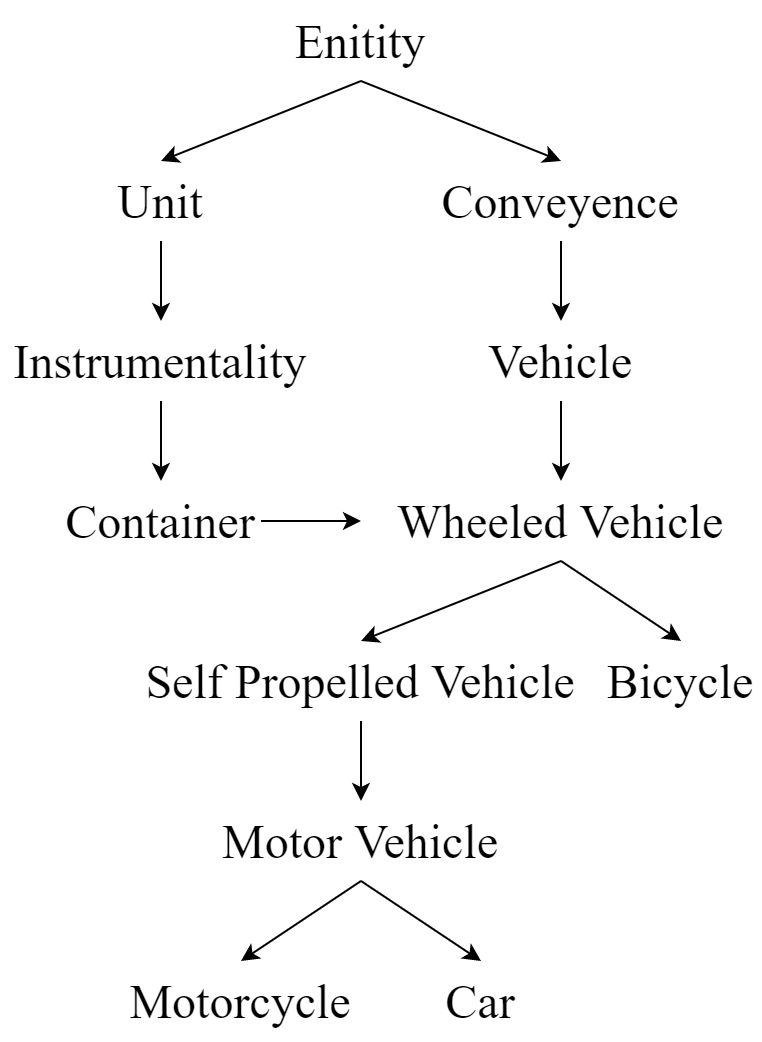
\includegraphics[width=250px]{WordNet.png}
  \caption{Hierarchical Structure from WordNet}
  \label{fig:wordnet}
\end{figure}

% 同義詞詞林由 Mei \emph{et al}. 完成,收錄了五萬三千多個詞。因年代久遠,許多用詞與現在已經差異很大,後來由 HIT 修編為同義詞詞林擴增版,擴增為七萬多個詞,並放在由 HIT 所建立的 Language Technology Platform Cloud 上供大家下載與研究。
\paragraph{}
Tongyici Cilin (or Chinese Synonym Forest, 同義詞詞林) written by Mei \emph{et al}. \cite{mei1983hit} in 1983, which has collected over 53k words. Nowadays, some words have become less used, and many modern words appear. Therefore, the Harbin Institute of Technology Information Retrieval Lab (HIT IR Lab)\footnote{http://ir.hit.edu.cn/} extended Tongyici Cilin to collected over 70k words and removed both the old words and the uncommon words. The Extended Tongyici Cilin is provided on the Language Technology Platform Cloud\footnote{https://www.ltp-cloud.com/} build by HIT for people to download and research.

\paragraph{}
The original Tongyici Cilin provides three levels of encoding to represent the synset. Level 1 using an upper letter, level 2 using a lower letter, and a two-digit number for level 3. There are additional level 4 and level 5 in Extended Tongyici Cilin to represent the finer granularity of the synsets as shown in Table \ref{table:tc_encoding}. An upper letter for level 4, and a two-digit number for level 5. The rank of the level is higher, the granularity is finer.

\paragraph{}
Figure \ref{fig:tc_sample} shows the examples of Tongyici Cilin. The level 1 encoding ``B'' is entity category, so the encoding of list begins with ``B'' is a list of entity words, like \texttt{Bf02A02=} and \texttt{Bg01A08@}. The level 1 encoding ``C'' is location category, so the encoding begins with ``C'' is a list of location words, like \texttt{Cb06E09@}.

\paragraph{}
The level 2 encoding ``Bf'' represents that the list of words is related to ``rain''. The level 3 encoding ``Bf02'' represents that the list of words is related to ``wind''. We can see that the encoding level is more similar, the group of the words is closer.

\paragraph{}
There is a category symbol follow by each encoding. ``='' represents that the words are synonyms. ``\#'' means that the words in the group are related. ``@'' indicates that the list only contains one word.

\begin{figure}[H]
  \centering
  \caption{Examples of Extended Tongyici Cilin}
  \begin{minipage}{\linewidth}
    \centering
    \setlength{\extrarowheight}{-3pt}
    \begin{tabular}{ll}
    Encoding & Words \\ \hline
    \texttt{Bf02A02=} & 大風\ 疾風\ 狂風\ 暴風\ 扶風 \\
    \texttt{Bf02A03=} & 颶風\ 颱風\ 強風\ 飈\ 強颱風 \\
    \texttt{Bf02B02=} & 雲氣\ 靄 \\
    \texttt{Bf04B02\#} & 朝霞\ 晚霞\ 煙霞 \\
    \texttt{Bg01A08@} & 溫水 \\
    \texttt{Cb06E09@} & 民間 \\
    \end{tabular}
    \label{fig:tc_sample}
  \end{minipage}
\end{figure}

\begin{table}[H]
  \centering
  \setlength{\extrarowheight}{-3pt}
  \begin{tabular}{|l|C{1.1cm}|C{1.1cm}|C{1.1cm}|C{1.1cm}|C{1.1cm}|C{1.1cm}|C{1.1cm}|C{1.1cm}|}
  \hline
  Digits & 1 & 2 & 3 & 4 & 5 & 6 & 7 & 8 \\ \hline
  Example & D & a & 1 & 5 & B & 0 & 2 & =\#@ \\ \hline
  Level & Lv1 & Lv2 & \multicolumn{2}{c|}{Lv3} & Lv4 & \multicolumn{2}{c|}{Lv5} &  \\ \hline
  \end{tabular}
  \caption{Extended Tongyici Cilin Encoding Table}
  \label{table:tc_encoding}
\end{table}

\paragraph{}
We use the WUP similarity \cite{wu-palmer-1994-verb} in WordNet to construct semantic features. The WUP similarity of synset is defined as Eq(\ref{eq:wup_synset}). $s_1$ and $s_2$ means the synset of a word. $lcs$ means the least common subsumer of the $s_1$ and $s_2$. $depth$ is the length of the synset to the root.

\begin{equation} \label{eq:wup_synset}
  wup_{synset}(s_1,s_2)=\frac{2\times depth(lcs)}{depth(s_1)+depth(s_2)}
\end{equation}

\paragraph{}
Since each word may have more than one synset, we defined the WUP similarity of word in Eq(\ref{eq:wup_word}). We calculate all the WUP similarities between all the synsets of the word $w_1$ and the word $w_2$. The maximum will be the word WUP similarity of $w_1$ and $w_2$.

\begin{equation} \label{eq:wup_word}
  wup_{word}(w_1,w_2)=\max\limits_{\substack{s_1\in synsets(w_1) \\ s_2\in synsets(w_2)}} wup_{synset}(s_1,s_2)
\end{equation}

\paragraph{}
We utilize NLTK (Natural Language Toolkit) \cite{nltk} to calculate the WUP similarity.

\paragraph{}
We use the Tongyici Cilin to build the lv5 similarity calculation system. The lv5 similarity of synset defined as Eq(\ref{eq:lv5_synset}). Given a synset $s_1$ and a synset $s_2$, we use $level$ to calculate the common level of $s_1$ and $s_2$, and then divide by five.

\begin{equation} \label{eq:lv5_synset}
  lv5_{synset}(s_1, s_2)=level(s_1,s_2)/5
\end{equation}

\paragraph{}
Since each word may linked by more than one synset in Tongyici Cilin, we defined the word-level lv5 similarity in Eq(\ref{eq:lv5_word}).

\begin{equation} \label{eq:lv5_word}
  lv5_{word}(w_1,w_2)=\max\limits_{\substack{s_1\in synsets(w_1) \\ s_2\in synsets(w_2)}} lv5_{synset}(s_1,s_2)
\end{equation}

\paragraph{}
% 因為中文的部份缺少完善的 WordNet 資源,而英文的部份則是缺少同義詞詞林的資源,所以這部份會透過 Cosine Similarity 來取代。
We lack a proper WordNet resource in Chinese since the existing Chinese WordNet is outmoded, it is unable to calculate the WUP similarity in Chinese since it will encounter too many missing words. And there is no similar resources of Tongyici Cilin in English, it is unable to calculate the lv5 similarity in English. They will be replaced with the cosine similarity. Given the word vectors $A$ and $B$, the cosine similarity is defined as Eq(\ref{eq:cos_sim}).

\begin{equation} \label{eq:cos_sim}
  sim_{cos}(A, B)=\frac{A\cdot B}{||A||\ ||B||}=\frac{\sum\limits^{n}_{i=1}A_iB_i}{\sqrt{\sum\limits^{n}_{i=1}A^2_i}\sqrt{\sum\limits^{n}_{i=1}B^2_i}}
\end{equation}

\paragraph{}
The average of the WUP similarity is defined in Eq(\ref{eq:average_wup}). The average of the lv5 similarity is defined in Eq(\ref{eq:average_lv5}). The cosine similarity is defined in Eq(\ref{eq:average_cos_sim}). $t_1$ and $t_2$ is the words of the premise and the hypothesis respectively. We sum the maximum and then divide by the total number of the words of $t_1$.

\begin{equation} \label{eq:average_wup}
  avg_{wup}(t_1,t_2)=\frac{1}{|t_1|}\sum\limits_{w_1\in t_1}\max\limits_{w_2\in t_2}wup_{word}(w_1, w_2)
\end{equation}

\begin{equation} \label{eq:average_lv5}
  avg_{lv5}(t_1,t_2)=\frac{1}{|t_1|}\sum\limits_{w_1\in t_1}\max\limits_{w_2\in t_2}lv5_{word}(w_1, w_2)
\end{equation}

\begin{equation} \label{eq:average_cos_sim}
  avg_{cos}(t_1,t_2)=\frac{1}{|t_1|}\sum\limits_{W_1\in t_1}\max\limits_{W_2\in t_2}sim_{cos}(W_1, W_2)
\end{equation}

\paragraph{}
Note that no matter in any type of similarity, we only consider the content words of the sentences.

\paragraph{}
The semantic features in English are listed as follows:

\begin{enumerate}
  \item[17.] average cosine similarity $(t_1)$
  \item[18.] average cosine similarity $(t_2)$
  \item[19.] average WUP similarity $(t_1)$
  \item[20.] average WUP similarity $(t_2)$
\end{enumerate}

\paragraph{}
The semantic features in Chinese are listed as follows:

\begin{enumerate}
  \item[17.] average cosine similarity $(t_1)$
  \item[18.] average cosine similarity $(t_2)$
  \item[19.] average lv5 similarity $(t_1)$
  \item[20.] average lv5 similarity $(t_2)$
\end{enumerate}

\subsubsection{Sentence Embedding} \label{sec:sent_emb}
\paragraph{}
% 因為句對間的蘊含關係有時並不需要用到整句話的資訊,只需要部份資訊,因此 Sentence Embedding 這種呈現 sentence features 的方法就是個不錯的選擇。Sentence Embedding 是由 Word Embedding 的向量計算而來,而關於 Word Embedding 的詳細敘述,請參考 Word Embedding 章節。在本論文中,我們選擇使用單純的總和平均做為計算 Sentence Embedding 的方法。
Another straightforward method to convert one sentence into one vector is to find the arithmetic mean of the embedding vectors of all the words in the sentence. The detailed discussion of word embedding is given in the Sec. \ref{section:word_embedding}.

\paragraph{}
After calculating sentence embedding vectors of the premise and the hypothesis in a pair from the RTE dataset, the real input to the neural network is the concatenation of these two embedding vectors.

\subsection{Word-Based Sequence Input}
\paragraph{}
The second kind of approaches to represent a sentence is to generate a sequence of word representations. For neural networks, a word is often represented as an embedding vector. The sequence of word embedding vectors can be the input of RNN or BERT.

\subsubsection{Original Word Sequence} \label{section:word_embedding}
\paragraph{}
% 在自然語言領域裡使用深度學習時,經常使用將每個字詞表達成一組向量的方法,將這組詞向量根據句子做排列而得到的詞向量序列做為神經網路的輸入層特徵。而在 RTE 任務裡,我們將 Premise 和 Hypothesis 串接起來,並在中間加入一個特殊 Token <SEP> 做為區隔。用來表達詞向量的方法有很多種,我們將在接下來的章節介紹這些語言模型。
When using deep learning in the field of natural language process, it is common to represent each word as a vector and combined it as a sequence of word vectors according to the order of the sentence, this word-based sequence will be the input features of the neural network. In the recognizing textual entailment task, we concatenated the sequence of word vectors of the premise and the hypothesis, a special token ``\texttt{[SEP]}'' will be put in the middle as the separator. There are many methods to represent the word embedding, we will introduce them in the following sections.

\subsubsubsection{Self-Trained Word Embedding}
\paragraph{}
% 與 Pre-trained Word Embedding 不同,Self-trained Embedding 通常做為神經網路的其中一個 Layer,並透過神經網路的梯度傳導機制不斷調整每個字詞的向量,根據任務的方向去學習適當的權重。Pre-trained Word Embedding 通常只會適合 pre-training 時所使用的文本領域,若是 pre-training 時的文本領域不夠廣泛或過於特殊,可能會對實驗效能有不好的影響。但因為 Self-trained Word Embedding 可以根據任務文本去進行彈性調整,所以在特定領域可能會有更好的表現,但也有可能因為資料數量不足的關係而使效能有所限制。
Different from the pre-trained word embedding, self-trained embedding usually use as a layer of a neural network and adjust each word vector through the backpropagation mechanism of the neural network. To the pre-trained word embedding, the suitable task is limited by the pre-training corpus. If the pre-training corpus is not common enough, it might have a bad influence on the experiments. The self-trained word embedding can do flexible adjustment according to the domain of the task text, therefore the performance may be better in a certain domain, but also may be limited by the data size of the training dataset.

\subsubsubsection{fastText}
\paragraph{}
fastText \cite{bojanowski2016enriching} is a library for efficient text classification and representation learning created by Facebook's AI Research (FAIR) lab. This library allows us to create word embedding with unsupervised learning algorithms, like skip-gram and continuous bag-of-word (CBOW). With this library, we train a word representation from Traditional Chinese Wikipedia, both in the version of skip-gram and CBOW. The dimension of the word embedding is 250.

\subsubsubsection{Google NNLM}
\paragraph{}
Google NNLM is provided by TensorFlow Hub\footnote{https://www.tensorflow.org/hub} which has many different language models that already be trained by a large corpus. We use the Chinese version of NNLM that trained on Simplified Chinese Google News 100B corpus and publish by Google\footnote{https://tfhub.dev/google/tf2-preview/nnlm-zh-dim128/1}. In order to fit the Traditional Chinese dataset, we convert the dictionary of the Google NNLM from Simplified Chinese into Traditional Chinese.
% BERT Language Model

\subsubsection{Similarity-Based Word Sequence} \label{section:csa}
% 指的是 CSA 但要講得比現在版本更清楚、要想像
\paragraph{}
We propose a new approach called similarity-based word sequence (SWS hereafter). This approach creates a new sequence of words (SWS) from two sentences according to the word alignment based on semantic similarity. The leading part of SWS contains semantically similar (aligned) words. The trailing part of SWS contains un-aligned (semantically dissimilar) words. The embedding vector of a word in SWS is the subtraction of the embedding vectors of the aligned words.

\paragraph{}
We expect SWS can be useful in RTE task. For a bidirectional entailment pair, most of the words can be aligned to their corresponding similar word, and the subtraction of their embedding vectors will be close to zero vector. For a forward entailment pair, the trailing part of SWS contains certain amount of un-aligned content words, therefore the entailment is one-directional. For an independent pair, both the premise and the hypothesis have content words that cannot be aligned.

\paragraph{}
If a contradiction pair is related to antonyms, at least one pair of un-aligned words are antonyms, and their vector subtraction can be identified by the neural network. If a contradiction pair is related to negations, one of the un-aligned words will be the negation word, and it may be recognized by the neural network.

\paragraph{}
Details and examples are given as follows. Figure \ref{fig:sws_b} shows an alignment result of a bidirectional entailment sentence pair, most of the words are aligned. Figure \ref{fig:sws_f} shows an alignment result of a forward entailment sentence pair, most of the words in the hypothesis are aligned, but some content words of the premise are not aligned. Figure \ref{fig:sws_i} shows an alignment result of an independence sentence pair, most of the words are un-aligned.

% B
% 有時候 生產商 會 在 鉛筆 的 一 端 裝上 橡皮擦
% 有時候 鉛筆 的 一 端 會 被 生產商 裝上 橡皮擦
\hspace*{-1.5in}
\begin{figure}[H]
  \centering
  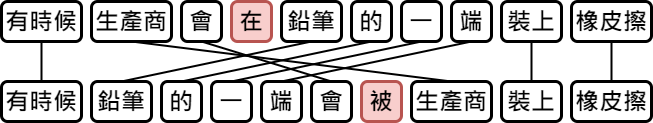
\includegraphics[scale=0.6]{SWS.B.png}
  \caption{SWS Bidirectional Entailment Example}
  \label{fig:sws_b}
\end{figure}

% F
% 約瑟夫·傅立葉 是 十九世紀 法國 數學家 、 物理學家
% 約瑟夫·傅立葉 是 物理學家
\hspace*{-1.5in}
\begin{figure}[H]
  \centering
  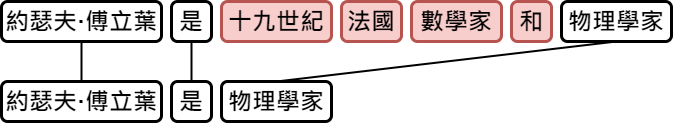
\includegraphics[scale=0.6]{SWS.F.png}
  \caption{SWS Forward Entailment Example}
  \label{fig:sws_f}
\end{figure}

% I
% 鉛筆 的 原型 可以 追溯 至 古羅馬 時代
% 羅馬人 發明 鉛筆
\hspace*{-1.5in}
\begin{figure}[H]
  \centering
  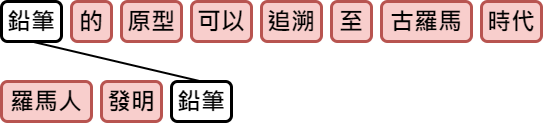
\includegraphics[scale=0.6]{SWS.I.png}
  \caption{SWS Independence Example}
  \label{fig:sws_i}
\end{figure}

\paragraph{}
Figure \ref{fig:sws_c_antonym} shows an alignment result of a contradiction sentence pair related to antonym. Un-aligned words are antonyms. Figure \ref{fig:sws_c_neg} shows an alignment result of a contradiction sentence pair related to negation, the negation word is un-aligned.

% C Antonym
% 東協 自由 貿易 區 於 1992年 提出
% 東協 自由 貿易 區 於 1992年 撤銷
\hspace*{-1.5in}
\begin{figure}[H]
  \centering
  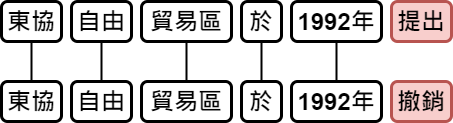
\includegraphics[scale=0.6]{SWS.C.Antonym}
  \caption{SWS Antonym Contradiction Example}
  \label{fig:sws_c_antonym}
\end{figure}

% C Negation
% 喬治·盧卡斯 最 著名 的 作品 是 《 星際 大戰 》 和 《 法櫃 奇兵 》 系列
% 喬治·盧卡斯 最 著名 的 作品 不 是 《 星際 大戰 》 和 《 法櫃 奇兵 》 系列
\begin{figure}[H]
  \centering
  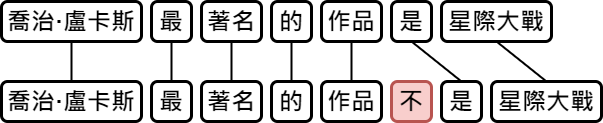
\includegraphics[scale=0.6]{SWS.C.Negation.png}
  \caption{SWS Negation Contradiction Example}
  \label{fig:sws_c_neg}
\end{figure}

% o align the words by calculating the cosine similarity between the premise and the hypothesis. We will have a argument ``similarity threshold'' to define if the two words will be aligned. We will decide the similarity threshold in the experiment of the threshold argument tuning.

\paragraph{}
We align the words based on the cosine similarity. We have a argument ``similarity threshold'' to control whether the words will be aligned. Figure \ref{fig:sim_threshold} shows an example that two different words are aligned since their cosine similarity is higher than the threshold. This threshold will be decide by the experiment of the argument tuning.

\hspace*{-1.5in}
\begin{figure}[H]
  \centering
  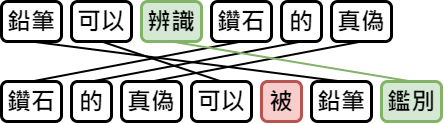
\includegraphics[scale=0.6]{Threshold.png}
  \caption{Alignment Result of Similarity-Based Word Sequence}
  \label{fig:sim_threshold}
\end{figure}

% 首先先計算兩句話的每個詞之間的 Cosine Similarity 建立一個 Similarity Table,然後從表中挑出相似數值最高的兩個詞,將 premise 的詞放入 list1 並將 hypothesis 的詞放入 list2,然後將這兩個詞從表中刪去,再繼續往下挑相似數值最高的兩個詞,直到該相似數值小於 Similarity Threshold 為止。接下來把 premise 剩下的詞一個一個放入 list1,每放一個詞到 list1 裡面,就在 list2 裡面放一個零,hypothesis 剩下的詞也是一樣的操作。最後將 list2 的值減去 list1 獲得最後的 CSA Features。
% To calculate the similarity-based word sequence, we will first calculate the cosine similarity of each word of two sentences to build a similarity table. Then picked up the word pair with the highest value of similarity, and put the word vector of the word from the premise sentence into $list_1$ and put the one from the hypothesis sentence into $list_2$. Then remove the two words from the similarity table. Repeat this step until the highest value of the similarity is lower than the similarity threshold. Next, we put the word vectors of the left words of the premise sentence into $list_1$ one by one. Every time we put a word vector into $list_1$, put a zero vector into $list_2$, and do the same operation to the left words of the hypothesis sentence. Therefore the two lists will remain the same size. After all, we use $list_2$ to minus $list_1$ to obtain the final ``SWS Features''.

\section{Training Data Expansion} \label{section:pseudo}

\paragraph{}
Many researches of deep learning in recent years mentioned that the scale of training data size has a huge impact on the performance of the system. RTE datasets are often constructed in a large scale. As we can see, the number of pairs in MNLI is 433k and the number of pairs in CNLI is 100k.

\paragraph{}
However, the number of pairs in the RITE2 training set is only 1,321 and it is only 581 in the RITE-VAL training set. The amount of the training data is extremely insufficient for deep learning. Therefore, we adopt two approaches, training using other NLI datasets and data expansion, to conquer the problem of data insufficiency.

\subsection{Expansion with Official Data} \label{sec:revlabel}
\paragraph{}
Two common methods to expand the training set among the RITE-VAL participants are adding reversed sentence pairs and previous RITE training sets.

\paragraph{}
The RITE-VAL training set provides reversed labels, which are the labels of sentence pairs when the roles of premise and hypothesis are exchanged. By reversing sentence pairs and assigning reversed labels to them, the training set can be expanded to its double size. We call this expanded dataset as RITE-Ex, which contains 1,103 sentence pairs.

\paragraph{}
We further combine the RITE-Ex dataset with the RITE2 training set and call it RITE-Ex2, which contains 2,292 sentence pairs.

\subsection{Training Using Other NLI Datasets} \label{section:add_other_nli}

% \paragraph{}
% We uses a larger training set constructed either for another domain, under a different definition of task, or in another language to pre-train a classifier, and then use the training set of the main task to fine-tune the classifier.

\paragraph{}
We use several available NLI datasets, including MNLI, CNLI, and OCNLI, as additional training data for building classifiers for RITE tasks. We also try to merge two datasets to become a larger training set.

\subsubsection*{Label Conversion}
\paragraph{}
Labels (entailment classes) defined in MNLI or CNLI datasets are different from the ones defined in RITE. MNLI and CNLI are ECN tasks, which means that the labels are ``entailment'', ``contradiction'', and ``neutral''. However, RITE tasks are BFCI tasks, which means that the labels are ``bidirectional entailment'', ``forward entailment'', ``contradiction'', and ``independence''. We need to find a method to convert ECN labels into BFCI labels.

\paragraph{}
Comparing the two label sets, ``contradiction'' is the same in both sets, and ``neutral'' can be map into ``independence'' directly. In order to decide whether an ``entailment'' pair is ``bidirectional entailment'' or ``forward entailment'', we try to build a good ECN classifier for each NLI dataset to automatically decide the entailment relations of the NLI pairs in the reverse direction.

\paragraph{}
Given an ``entailment'' pair, the two sentences in the pair are exchanged, i.e. the premise becomes the hypothesis and the hypothesis becomes the premise. We then use the ECN classifier to decide its label. If it is ``entailment'', it means that the entailment is in both direction, thus the final label is ``bidirectional entailment''. On the other hand, if the label of the reversed pair is ``neutral'', it means that the entailment only in one direction, thus the final label is ``forward entailment''. In rare cases, the reversed pair is mis-classified into ``contradiction''. We ignore such result and assign the label of the pair as ``forward entailment''.

\subsubsection*{Multilinguality}
\paragraph{}
Note that these datasets were constructed in different languages. MNLI is in English, and both CNLI and OCNLI are in Chinese. Since CNLI and OCNLI are in the same language with RITE, the monolingual language models can be used for pre-training, such as our pre-trained Chinese word embedding model or BERT.

\paragraph{}
To use training sets written in different languages, we need to choose a multilingual language model. Fortunately, BERT also provide a multilingual version. We can use the multilingual BERT to train a model by MNLI, a dataset in English, and then fine-tune the model with a RITE training set written in Chinese.

\subsubsection*{Two-Step Pre-Training}
\paragraph{}
When using a single NLI dataset as the additional training data, we first pre-train the model with this NLI dataset and then fine-tune with the RITE training sets.

\paragraph{}
When both MNLI and CNLI are used, two approaches to combine these two datasets are proposed. The first approach is to merge MNLI and CNLI to become a larger dataset. The second approach is two-step pre-training. We first pre-train the model with MNLI, and then pre-train the model with CNLI. These pre-trained models are further fine-tuned with the RITE training sets.

\paragraph{}
The fine-tuning and evaluation steps are performed in the way of 10-fold cross-validation. The overall performance on the training set for each BFCI classes is the micro-averaging F1-score of 10 folds. The test set is predicted in every fold and the overall performance on the test set is the macro-averaging F1-score of 10 folds.

\subsection{Generation-Based Data Expansion}
% 我們嘗試使用大量的虛擬資料來改進模型的效能,虛擬資料的產生方式則有規則式改寫與 GPT-2 模型生成兩種。這兩種方法會對四個標籤都產生等量的資料,並根據 MNLI 的資料量,各產生 400k 組句對。在接下來的章節會介紹產生虛擬資料的細節。
\label{section:pseudo_dataset}
\paragraph{}
We attempt to automatically create large-scale pseudo datasets to improve the performance of textual entailment recognition. We propose two approaches to generate the pseudo data, including rule-based rewriting and GPT-2 generation. Both methods will generate equal amount of data for four labels. To be comparable with MNLI, the set of pairs in each label will be expanded to 400k.

\subsubsection{Rule-Based RTE Pair Generation}
% \subsubsection{CIRB}
% CIRB, Synonym Dictionary, Antonym Dictionary, Negation Words
% 首先我們先介紹產生虛擬訓練資料會需要用到的資源。因為產生虛擬資料的方法基本上是透過改寫句子得來的,而改寫規則未必能夠適用於任何句子上,因此我們需要有足夠大量的文章才能確保生成的句子數量是充足的。CIRB (Chinese Information Retrieval Benchmark) 是一份來自 NTCIR 2 資訊檢索子任務的測試集,蒐集了 1998 年到 2005 年間五家線上新聞媒體的新聞文章資料,總共 280 萬篇文章,每篇文章的長度平均為 560 個字,包含的領域廣泛分佈於政治、財經、體育、娛樂、科技、國際等。且 RITE 資料集本身也有一些句子是來自於新聞文章,所以我們認為 CIRB 是一個相當合適的資料集。
\label{para:cirb}
\paragraph{}
We design several rewriting rules to generate RTE pairs, including synonym/antonym substitution and negation insertion. Long sentences can be further divided to create new sentences. These methods are explained as follows.

\subsubsubsection*{Synonym/Antonym substitution}
\paragraph{}
Given a sentence in Chinese natural language, we randomly pick a word in the sentence which have synonyms or antonyms in the dictionary, and replace the word with one of its synonyms or antonyms randomly.

\paragraph{}
Assume that a word $w$ in a sentence $S$ is substituted and the sentence $S$ becomes $S'$, if the word $w$ is substituted with its synonym, $S$ and $S'$ still have the same meaning, thus $(S,S')$ is a ``bidirectional entailment'' pair. On the other hand, if the word $w$ is substituted with its antonym, $S$ and $S'$ will have antonymous meanings, thus $(S,S')$ is a ``contradiction'' pair.

\paragraph{}
We use the synonym dictionary and the antonym dictionary to generate the pseudo training data. The synonym dictionary can be built by using the Tongyici Cilin base on the well-organized synonym encoding. And the Academia Sinica Bilingual Ontological WordNet (Sinica BOW) \cite{huang2004sinica} can be used to build the antonym dictionary.

\paragraph{}
Sinica BOW is a thesauri that integrates the English WordNet 1.6 and the Chinese WordNet. Figure \ref{fig:bow} shows the example data of Sinica BOW. We can see that the record of the Sinica BOW is built based on the synset offset of WordNet. We can easily build the Chinese antonym dictionary by the antonym information in WordNet with these mapping records from Sinica BOW.

\begin{figure}
  \centering
  \caption{Example of the Academia Sinica Bilingual Ontological WordNet}
  \begin{minipage}{\linewidth}
    \begin{lstlisting}[language=XML]
    <Record Count="171509">
      <EnglishLemma>deep</EnglishLemma>
      <POS>Adverb</POS>
      <WordNetSynsetOffset Version="1.6">00300307</WordNetSynsetOffset>
      <EnglishFrequancyRank>#通用詞彙#</EnglishFrequancyRank>
      <ChineseTransList>
        <ChineseTrans>
          <ChineseLemma>#深入地#</ChineseLemma>
        </ChineseTrans>
      </ChineseTransList>
    </Record>
    <Record Count="171510">
      <EnglishLemma>deep</EnglishLemma>
      <POS>Adjective</POS>
      <WordNetSynsetOffset Version="1.6">00654761</WordNetSynsetOffset>
      <EnglishFrequancyRank>#通用詞彙#</EnglishFrequancyRank>
      <ChineseTransList>
        <ChineseTrans>
          <ChineseLemma>#深的#</ChineseLemma>
        </ChineseTrans>
      </ChineseTransList>
    </Record>
    \end{lstlisting}
  \end{minipage}
  \label{fig:bow}
\end{figure}

\subsubsubsection*{Negation Insertion}
\paragraph{}
Given a sentence with no negation words, we try to find the best position to insert a negation word according to a part-of-speech trigram probabilistic model. The list of negation words comes from
Tongyici Cilin.

\paragraph{}
To apply this rule, we have to prepare a negation-related part-of-speech trigram probabilistic model. First, we collect sentences with negation words in a large corpus. Second, these sentences are POS-tagged by CKIP tagger \footnote{https://github.com/ckiplab/ckiptagger}\cite{Li_Fu_Ma_2020} and all words except negation words are replaced with their POS. Trigrams where the second word is a negation word are extracted for further calculation. Note that the marks of sentence boundaries are added at the beginning and in the end of sentences before trigram extraction.

% negation-context frequency
\paragraph{}
Bigrams consisting of the first and the third POS in these negation-centered trigrams are extracted and counted. We define the frequency of such a bigram as its \textbf{\emph{negation-context frequency}}. Given a POS-tagged sentence, an occurrence of a POS bigram with a high negation-context frequency indicates that it is likely to appear a negation word in the middle of the bigram. We simply choose the POS bigram with a highest negation-context frequency and insert a negation word in the middle. The sentences before and after the negation insertion form a new ``contradiction'' pair.

\paragraph{}
The choice of the inserted negation word is random but according to the ratio of the occurrence of negation words. For a POS bigram, we collect the negation-centered trigrams which generate this POS bigram, and count the frequency of each negation word appearing in the center. The probability of a negation word to be inserted is proportional to its frequency in these trigrams.

% ('Na', 'Nb'): '否': 90, '非': 10
% ('Na', 'Nc'): '否': 10, '非': 990

\subsubsubsection*{Sentence Splitting}
\paragraph{}
We use a straightforward method to create ``forward entailment'' pairs. That is, we choose sentences containing one or more commas and divide it into several sub-sentences according to the commas. The original sentence and any one of its sub-sentences can produce a ``forward entailment'' pair.

\paragraph{}
This method can be also applied to the new pairs generated by the previous two rules. Given a rule-generated pair $(t_1,t_2)$, $t_1$ can be paired with any sub-sentence of $t_2$ to become a new RTE pair. If the sub-sentence contains a synonym, the label of the new pair is ``forward entailment''. If the sub-sentence contains an antonym, the label of the new pair is ``contradiction''. If the sub-sentence contains a newly inserted negation word, the label of the new pair is ``contradiction''. Otherwise, the label of the new pair is ``forward entailment''.

\subsubsubsection*{Random Selection}
\paragraph{}
Finally, we randomly choose two sentences from the large corpus to produce a new RTE pair and assign its label as ``independence''. Table \ref{example:sim_nli_rule_based} shows the examples of sentence pair generated by rule-based generation.

\paragraph{}
\paragraph{}
Obviously, we need a large corpus to pick sentences for RTE pair generation and to measure the negation-context frequencies. We merge all the CIRB corpora to become a large corpus for this purpose.

% \paragraph{}
% First, we introduce the resources used in the generation of pseudo training data. Most of the generated data come from the modification of sentences and the rewriting rules may not be applied to any sentences, so we need to ensure the number of the articles is enough to generate sufficient sentences.

\paragraph{}
The CIRB (Chinese Information Retrieval Benchmark) \cite{chen2001cirb} dataset is a test collection of the Chinese information retrieval tasks of NTCIR 2 which collected the news articles released from the websites of Chinatimes\footnote{https://www.chinatimes.com/}, Chinatimes Commercial\footnote{https://ctee.com.tw/}, Chinatimes Express, Central Daily News, and China Daily News during 1998 to 2005.

\paragraph{}
There are in total 2.8 million articles with an average length of 560 characters. The domains covered are widely distributed in politics, finance, sports, entertainment, technology, and international. Besides, the part of sentences in the RITE dataset also comes from the news article. We believe that the CIRB collection is a suitable corpus for our purpose.

\begin{table}[H]
  \centering
  \setlength{\extrarowheight}{-3pt}
  \caption{Example of Sentence Pairs Generated by Rule-Based Methods}
  \label{example:sim_nli_rule_based}
  \begin{tabular}{|L{3.6cm}|L{10.05cm}|C{1cm}|}
  \hline
  \multicolumn{1}{|c|}{Method} & \multicolumn{1}{c|}{Sentence Pair} & Label \\ \hline
  \multirow{2}{*}{Synonym} & 失控所致或營造而成,差異極大 & \multirow{2}{*}{B} \\ \cline{2-2}
   & 失控所致或營造而成,反差極大 &  \\ \hline
  \multirow{2}{*}{Antonym} & 即日起上市,可預約宅配 & \multirow{2}{*}{C} \\ \cline{2-2}
   & 即日起上市,不許預約宅配 &  \\ \hline
  \multirow{2}{*}{Negative} & 相較之下,台灣藝術家以公共藝術文化輸出的案例卻未聽聞 & \multirow{2}{*}{C} \\ \cline{2-2}
   & 相較之下,台灣藝術家以非公共藝術文化輸出的案例卻未聽聞 &  \\ \hline
  \multirow{2}{*}{Splitting} & 也許真的自古英雄多寂寞,女人也不例外 & \multirow{2}{*}{F} \\ \cline{2-2}
   & 也許真的自古英雄多寂寞 &  \\ \hline
  \multirow{2}{*}{Synonym \&   Splitting} & 失控所致或營造而成,差異極大 & \multirow{2}{*}{F} \\ \cline{2-2}
   & 反差極大 &  \\ \hline
  \multirow{2}{*}{Antonym \&   Splitting} & 即日起上市,可預約宅配 & \multirow{2}{*}{C} \\ \cline{2-2}
   & 不許預約宅配 &  \\ \hline
  \multirow{2}{*}{Negative \&   Splitting} & 相較之下,台灣藝術家以公共藝術文化輸出的案例卻未聽聞 & \multirow{2}{*}{C} \\ \cline{2-2}
   & 台灣藝術家以非公共藝術文化輸出的案例卻未聽聞 &  \\ \hline
  \multirow{2}{*}{Random Selection} & 也許真的自古英雄多寂寞,女人也不例外 & \multirow{2}{*}{F} \\ \cline{2-2}
   & 這個週期「魔咒」,誰也掙脫不了 &  \\ \hline
  \end{tabular}
\end{table}

\subsubsection{GPT-2 Generation}
% GPT-2 \cite 是由 OpenAI 所開發的一個自然語言產生模型,在機器翻譯、問答、總結和文本產生都有相當出色的表現。而透過 GPT-2 模型產生虛擬資料的這個實驗,我們參考了 _ 論文中的做法,從 Corpus 中隨機挑選句子,並將非內容詞去除,只留下內容詞做為「head seed」,然後將完整的句子拼接在 head seed 後面,目的是訓練 GPT-2 模型在餵入這些內容詞後,可以產生完整的句子。在適當的訓練下,對 GPT-2 模型餵入相同的內容詞做為 head seed 可以產生不同但相似的句子。
\paragraph{}
GPT-2 \cite{radford2019language} is a natural language generation model created by OpenAI. It has an excellent performance in machine translation, question answering, summarization, and text generation. The GPT-2 generation method of the simulation dataset is based on Hegde \emph{et al}. \cite{hegde2020unsupervised}.

\paragraph{}
We randomly picked sentences from the corpus and removed the non-content word, only remain the content words as the seeds of GPT-2. Then we concatenated the original sentence after the seeds. We use special tokens \texttt{[CLS]} and \texttt{[SEP]} to surround the seed. Therefore, the model can distinguish the boundary of the seeds and the sentence.

\paragraph{}
Our purpose is to train the GPT-2 model that can generate a complete sentence including the words of the seeds. With proper training, the GPT-2 model can generate different but similar sentences from the same seeds.

% 我們保留訓練資料中的原句做為 Premise,並使用相同的 head seed 產生一個句子做為 Hypothesis ,這樣獲得的句對可以標記為 B。接下來,我們透過更換 head seed 的內容詞來產生其他不同標記的句對。從 head seed 中隨機挑選兩個詞並互換位置,這樣產生的句對為 B。將 head seed 中的部份內容詞去除,這樣產生的句對為 F。從 head seed 中隨機挑選一個內容詞變成反義詞,這樣產生的句對為 C。隨機插入一個否定詞在 head seed 裡面,產生出來的句對為 C。只保留一個 head seed 的內容詞,並隨機放入其他內容詞,產生出來的句對為 I。
\paragraph{}
We keep the original sentence of the training example as the premise sentence and use the same seeds from the training example to generate a new sentence as the hypothesis sentence. These sentence pairs will be labeled as ``bidirectional''.

\paragraph{}
Next, we generate sentences for different labels by changing the word of seeds. We randomly pick one word and replace it with synonym. The generated sentence pairs will be labeled as ``bidirectional''. We randomly pick two words of seeds and exchanged their position. The generated sentence pairs will be labeled as ``bidirectional''.

\paragraph{}
We randomly remove one to three words of seeds, the generated sentence pairs will be labeled as ``forward entailment''. We randomly pick one content word and replace it with an antonym, the generated sentence pairs will be labeled as ``contradiction''.

\paragraph{}
We randomly insert a negation word in seeds, the generated sentence pairs will be labeled as ``contradiction''. At last, only remain one content word of seeds and put three to ten random words within, the generated sentence pairs will be labeled as ``independence''. Table \ref{example:GPT-2_pseudo} shows the examples of the GPT-2 pseudo sentences.

\begin{table}[H]
  \centering
  \setlength{\extrarowheight}{-3pt}
  \caption{Example of Sentence Generated by GPT-2}
  \label{example:GPT-2_pseudo}
  \begin{tabular}{|L{2cm}|L{5cm}|L{6.2cm}|c|}
  \hline
  \multicolumn{1}{|c|}{Method} & \multicolumn{1}{c|}{Generation Seed} & \multicolumn{1}{c|}{Generated Sentence} & Label \\ \hline
  Original & 目前\ 消失\ 提出\ 質疑 & 目前是否已經消失,一度提出質疑。 & - \\ \hline
  Same & 目前\ 消失\ 提出\ 質疑 & 並對目前已消失的提出質疑。 & B \\ \hline
  Exchange & 消失\ 目前\ 提出\ 質疑 & 是否在消失,以目前似乎一再提出質疑。 & B \\ \hline
  Synonym & 當下\ 消失\ 提出\ 質疑 & 當下並未消失,她提出質疑。 & B \\ \hline
  Remove & 目前\ 提出\ 質疑 & 目前也曾提出質疑。 & F \\ \hline
  Antonym & 目前\ 出現\ 提出\ 質疑 & 不過,目前沒有出現提出質疑。 & C \\ \hline
  Negation & 目前\ 非\ 消失\ 提出\ 質疑 & 目前雖非消失,卻提出質疑。 & C \\ \hline
  Random & 出發\ 能力\ 質疑\ 表達\ 清楚 & 再出發的能力,他質疑是否能表達清楚。 & I \\ \hline
  \end{tabular}
\end{table}

% 我們使用 CIRB 做為 Corpus,並根據四個標籤平均生成資料集,每個標籤下的每一種方法也同樣生成平均數量的資料。規則式與 GPT-2 根據 MNLI 的資料集規模,各自生成四十萬組句對,總共生成八十萬組句對。
\paragraph{}
We generate the dataset equally according to the four labels, each generation method also generates an equal number of data under each label. Both rule-based and GPT-2 generate 400k sentence pairs respectively. Both scale of the training set is similar to MNLI, result in an 800k sentence pairs pseudo training dataset. Table \ref{table:pseudo_training_data_dist} shows the distribution of the pseudo training dataset.

\begin{table}[H]
  \centering
  \setlength{\extrarowheight}{-3pt}
  \begin{tabular}{|l|l|c|r|c|}
  \hline
  \multicolumn{1}{|c|}{System} & \multicolumn{1}{c|}{Method} & Label & \multicolumn{1}{c|}{Number} & Total \\ \hline
  \multirow{10}{*}{Rule-Based} & Synonym & B & 100k & \multirow{10}{*}{400k} \\ \cline{2-4}
   & Antonym & C & 25k &  \\ \cline{2-4}
   & Negation Word & C & 25k &  \\ \cline{2-4}
   & Antonym and Split (1) & C & 25k &  \\ \cline{2-4}
   & Negation Word and Split (1) & C & 25k &  \\ \cline{2-4}
   & Synonym and Split & F & 33k &  \\ \cline{2-4}
   & Antonym and Split (2) & F & 33k &  \\ \cline{2-4}
   & Negation Word and Split (2) & F & 33k &  \\ \cline{2-4}
   & Radom Pick & I & 50k &  \\ \cline{2-4}
   & Random Split & I & 50k &  \\ \hline
  \multirow{7}{*}{GPT-2} & Same Seed & B & 33k & \multirow{7}{*}{400k} \\ \cline{2-4}
   & Synonym & B & 33k &  \\ \cline{2-4}
   & Exchange Position & B & 33k &  \\ \cline{2-4}
   & Random Remove & F & 100k &  \\ \cline{2-4}
   & Antonym & C & 50k &  \\ \cline{2-4}
   & Negation Word & C & 50k &  \\ \cline{2-4}
   & Remain One & I & 100k &  \\ \hline
  \end{tabular}
  \caption{The Pseudo Training Data Distribution}
  \label{table:pseudo_training_data_dist}
\end{table}

\section{Experiments} \label{section:experiments}
\subsection{Datasets and Evaluation Metrics}
\paragraph{}
The main experimental datasets in this thesis are RITE2 and RITE-VAL datasets, both with training sets and test sets. They are designed for Traditional Chinese RTE BFCI tasks. We use BERT Chinese version and BERT multilingual version to train classifiers.

\paragraph{}
Several NLI datasets designed for ECN tasks are used as additional training data. Their labels are converted into BFCI as described in Sec. \ref{section:add_other_nli}. These datasets are:

\begin{itemize}
  \item MNLI, an English dataset, for BERT multilingual version only
  \item CNLI, the Traditional Chinese version (as described in Sec. \ref{sec:cnli})
  \item OCNLI, the Traditional Chinese version (as described in Sec. \ref{sec:ocnli})
\end{itemize}

\paragraph{}
% 在 RITE 的實驗中,我們對 Training Set 進行 10-Fold Cross-validation,並計算這十個 Fold 的 Micro F1-Score 做為評估結果之一。而測試集的部份則以 10-Fold 產生出來的 10 個權重各評估一次並取平均做為 Test F1-Score。
When experimenting on RITE training sets, we evaluate the systems by 10-fold cross-validation. If additional NLI datasets are used to pre-train classifiers as described in Sec. \ref{section:add_other_nli}, the pre-training step uses the whole NLI datasets and the fine-tuning step is implemented in the cross-validation way.

% In the experiments of RITE, we do the 10-fold cross-validation to the training set and calculate the micro F1-score as one of the evaluation results. We evaluate the test set by each model weight of the ten folds, then take the average as test F1-score.

\paragraph{}
The evaluation metrics of RTE are precision, recall, and F1-score of each RTE category (BFCI). The overall performance is measured in the macro-averaging F1-scores of all the categories. They are defined as follows.

\begin{equation}
  Precision=\frac{N_{correct}}{N_{predicted}}
\end{equation}

\begin{equation}
  Recall=\frac{N_{correct}}{N_{target}}
\end{equation}

\begin{equation}
  F1=\frac{2\times Precision\times Recall}{Precision+Recall}
\end{equation}

\begin{equation}
  macroF1=\frac{1}{|C|}\sum_{c\in C}F1_c
\end{equation}

\paragraph{}
where $N_{correct}$ is the number of corrected labeled sentence pairs, $N_{predicted}$ is the number of sentence pairs predicted in one RTE category, $N_{target}$ is the real number of sentence pairs belonging to one RTE category, $C$ is the set of all RTE categories, and $F1_{c}$ is the F1-score of Category $c$.

% \paragraph{}
% To compare the experiments of the ECN tasks with the other systems, we use accuracy as the evaluation formula of the ECN tasks.

% \paragraph{}
% To understand the impact of the characters of the Traditional and the Simplified, we use OpenCC\footnote{https://github.com/BYVoid/OpenCC} which available as a python package to convert CNLI and OCNLI into CNLI-CT and OCNLI-CT. The original CNLI and OCNLI in Simplified Chinese will be called CNLI-CS and OCNLI-CS.

\subsection{Machine Learning Feature Experiments}
% 首先我們重製了 Liu 等人的 SVM 實驗,並與 MLP 做比較。在 Scikit-Learn 套件中提供了四個 Kernel: RBF, Linear, Sigmoid, and Poly,所以我們先比較了不同的 SVM Kernel。
% 在 Liu 等人的實驗中,分別將 Lexical (lex), Syntactic (syn), Word Similarity (wn), 與 Synonym Forest (cl) 各自去除,來測試哪個特徵對實驗結果的影響較大。而在 MLP 的實驗中,我們也做了相同的步驟。
% 接下來,我們嘗試用基本的 RNN Model 來進行實驗。RNN 的部份測試了 LSTM 與 GRU 以及各自加上 Attention 的效果,在 Word Embedding 的部份則測試了 Self-trained, fastText CBOW, fastText Skip-gram, 與 GoogleNNLM。其結果如表:(待補)
% (st/ftCBOW/ftSG/g x LSTM/GRU x with/without Attention)
% 在這個實驗的基礎上,我們將 ML Features 結合到 RNN Model 裡面。我們將 RNN Encoder 的 Output 與 ML Features 做 Concatenate 後再進行分類,其結果如表(待補)
% 而在本論文中,我們提出了 CSA 方法,並將 CSA 特徵放入 RNN Model,也分別測試了與 ML Features 或 Word Embedding 做結合的實驗,其結果如表:(待補)
% \paragraph{}
% To cross-compare the performance of datasets, we first extended the RITE-VAL with reversed labels to generate RITE-VAL-REV and mixed RITE2 with RITE-VAL-REV to generate RITE-VAL-REV-2. So we have RITE2, RITE-VAL, RITE-VAL-REV, and RITE-VAL-REV-2 to be used as the training sets. The test sets of RITE2 and RITE-VAL will be called as RITE2-TEST and RITE-VAL-TEST.

\paragraph{}
As described in Sec. \ref{section:ml_features}, machine learning feature vectors can be one kind of input to a neural network. We use MLP to construct such kind of classifiers and compare them with machine learning classifiers built by SVM with different kernels such as radial basis function (RBF), linear, sigmoid, and polynomial functions provided in the Scikit-Learn package.

\paragraph{}
The results are shown in Table \ref{svm_kernel}. We can see that the performance of kernel RBF outperforms all the other kernels except the RITE2 test set. Therefore, the RBF kernel will be chosen as the main kernel in the following experiments.

\begin{table}[H]
  \centering
  \setlength{\extrarowheight}{-3pt}
  \caption{Comparison of SVM and MLP}
  \label{svm_kernel}
  \begin{tabular}{|l|C{1.5cm}|C{1.5cm}|C{1.5cm}|C{1.5cm}|}
  \hline
  \multicolumn{1}{|c|}{\multirow{2}{*}{SVM Kernel}} & \multicolumn{2}{c|}{RITE2} & \multicolumn{2}{c|}{RITE-VAL} \\ \cline{2-5}
  \multicolumn{1}{|c|}{} & \multicolumn{1}{c|}{Training} & \multicolumn{1}{c|}{Test} & \multicolumn{1}{c|}{Training} & \multicolumn{1}{c|}{Test} \\ \hline
  RBF & 0.5336 & 0.4227 & 0.3840 & \textbf{0.3678} \\ \hline
  Linear & 0.5382 & 0.4594 & 0.3516 & 0.3177 \\ \hline
  Sigmoid & 0.3335 & 0.2973 & 0.2844 & 0.2822 \\ \hline
  Poly & 0.5474 & 0.4241 & 0.3437 & 0.2832 \\ \hline \hline
  MLP & \textbf{0.5913} & \textbf{0.4625} & \textbf{0.4220} & 0.3542 \\ \hline
  \end{tabular}
\end{table}

\subsection{Sentence Embedding Experiment}
% 在 Sentence-based embedding 的實驗中,我們將 Self-Trained Word Embedding, fastText CBOW, fastText Skip-gram 與 Google NNLM 等四種 NNLM 分別進行測試,sentence embedding 的算法為 word embedding 的平均,其結果如表。可見 fastText CBOW 的效果較好,我們認為這是 CBOW 的特性使得這個 NNLM 相當適合進行 Sentence Embedding 的實驗。
\paragraph{}
As described in Sec. \ref{sec:sent_emb}, the embedding vector of a sentence can be the arithmetic mean of all the word embeddings in the sentence. We test the four word embedding models introduced in Sec. \ref{section:word_embedding} to generate sentence embeddings.

\paragraph{}
The results are shown in Table \ref{result:sent_emb_nnlm}. We can see that the performance of the word embedding model built by fastText CBOW method is the best. However, the best performance is quite low comparing to other experiments introduced later.

\begin{table}[H]
  \centering
  \setlength{\extrarowheight}{-3pt}
  \caption{Results of Sentence Embedding Experiment}
  \label{result:sent_emb_nnlm}
  \begin{tabular}{|l|C{1.5cm}|C{1.5cm}|C{1.5cm}|C{1.5cm}|}
  \hline
  \multicolumn{1}{|c|}{\multirow{2}{*}{Word Embedding}} & \multicolumn{2}{c|}{RITE2} & \multicolumn{2}{c|}{RITE-VAL} \\ \cline{2-5}
  \multicolumn{1}{|c|}{} & \multicolumn{1}{c|}{Training} & \multicolumn{1}{c|}{Test} & \multicolumn{1}{c|}{Training} & \multicolumn{1}{c|}{Test} \\ \hline
  Self-Trained & 0.2711 & 0.1445 & 0.1382 & 0.1000 \\ \hline
  fastText CBOW & \textbf{0.3818} & 0.2755 & \textbf{0.3335} & \textbf{0.2551} \\ \hline
  fastText Skip-Gram & 0.3623 & \textbf{0.2762} & 0.2631 & 0.1550 \\ \hline
  Google NNLM & 0.1851 & 0.2019 & 0.2363 & 0.1874 \\ \hline
  \end{tabular}
\end{table}

\subsection{Word Embedding Experiments}
\paragraph{}
In Sec. \ref{section:word_embedding}, four kinds of word embedding models are introduced. Table \ref{result:nnlm_comparison} lists the performance of RNN classifiers using these word embedding models. Each RNN classifier is composed of three layers which are a GRU layer, an attention layer, and a fully-connected layer.

\paragraph{}
As shown in Table \ref{result:nnlm_comparison}, classifiers using the word embedding models trained by fastText with the skip-gram method on Chinese Wikipedia outperform the other word embedding models, except in the experiment of the RITE-VAL training set where the self-trained embedding model is the best.

\begin{table}[H]
  \centering
  \setlength{\extrarowheight}{-3pt}
  \caption{Comparison of Different Word Embeddings}
  \label{result:nnlm_comparison}
  \begin{tabular}{|l|C{1.5cm}|C{1.5cm}|C{1.5cm}|C{1.5cm}|}
  \hline
  \multicolumn{1}{|c|}{\multirow{2}{*}{Word Embedding}} & \multicolumn{2}{c|}{RITE2} & \multicolumn{2}{c|}{RITE-VAL} \\ \cline{2-5}
  \multicolumn{1}{|c|}{} & Training & Test & Training & Test \\ \hline
  Self-Trained & 0.3610 & 0.2453 & \textbf{0.4280} & 0.2108 \\ \hline
  fastText CBOW & 0.3670 & 0.2420 & 0.3790 & 0.2260 \\ \hline
  fastText Skip-Gram & \textbf{0.3731} & \textbf{0.2587} & 0.4227 & \textbf{0.2351} \\ \hline
  Google NNLM & 0.3086 & 0.2346 & 0.2862 & 0.2066 \\ \hline
  \end{tabular}
\end{table}

\paragraph{}
Of course there are many ways to construct a RNN classifier. We further investigate the effect of using different kinds of RNN, using an attention layer, and the position of the attention layer, and compare them with BERT.

\paragraph{}
The effect of attention layers is investigated by evaluating the RNN classifiers listed in Table \ref{result:nn_types_comparison}. The first column lists the models of the RNN classifiers, where ``R'' denotes ``GRU layer'', ``A'' denotes ``attention layer'', ``D'' denotes ``fully-connected dense layer'', and the order of the letters indicates the order of the layers.

\paragraph{}
As shown in Table \ref{result:nn_types_comparison}, the best system is the RAD model where an attention layer is added after a GRU layer. We use this model for all RNN classifiers hereafter.

\begin{table}[H]
  \centering
  \setlength{\extrarowheight}{-3pt}
  \caption{Comparison of the Effect of Attention Layers}
  \label{result:nn_types_comparison}
  \begin{tabular}{|l|C{1.5cm}|C{1.5cm}|C{1.5cm}|C{1.5cm}|}
  \hline
  \multicolumn{1}{|c|}{\multirow{2}{*}{Model}} & \multicolumn{2}{c|}{RITE2} & \multicolumn{2}{c|}{RITE-VAL} \\ \cline{2-5}
  \multicolumn{1}{|c|}{} & Training & Test & Training & Test \\ \hline
  RAD & \textbf{0.3731} & \textbf{0.2587} & \textbf{0.4227} & \textbf{0.2351} \\ \hline
  ARD & 0.3705 & 0.2356 & 0.3986 & 0.1995 \\ \hline
  RD & 0.3728 & 0.2387 & 0.3868 & 0.2014 \\ \hline
  AD & 0.3674 & 0.2480 & 0.3359 & 0.1714 \\ \hline
  \end{tabular}
\end{table}

% 比較 RNN Types
\paragraph{}
% RNN 有多種變形,藉由 Tensorflow API 我們可以使用三種基本的 RNN 形式:Vanilla RNN, LSTM, 與 GRU,我們將這三種 RNN 做比較,得到表的結果。可見 GRU 與 LSTM 的效果差距很小,因為 GRU 所需消耗的訓練資源比較低,所以我們選擇 GRU 做為主要的 RNN Layer。
Table \ref{result:rnn_types} shows the performance of different types of recurrent neural networks, including vanilla RNN, LSTM, and GRU. The best choice is GRU, since it achieves better performance in most cases.

\paragraph{}
We also compare the BERT model with these three types of RNN classifiers. We can see that BERT outperforms all the RNN classifiers.

\begin{table}[H]
  \centering
  \setlength{\extrarowheight}{-3pt}
  \caption{Results of the Different Neural Networks}
  \label{result:rnn_types}
  \begin{tabular}{|l|C{1.5cm}|C{1.5cm}|C{1.5cm}|C{1.5cm}|}
  \hline
  \multicolumn{1}{|c|}{\multirow{2}{*}{Neural Network}} & \multicolumn{2}{c|}{RITE2} & \multicolumn{2}{c|}{RITE-VAL} \\ \cline{2-5}
  \multicolumn{1}{|c|}{} & Training & Test & Training & Test \\ \hline
  Vanilla RNN & 0.3278 & 0.2519 & 0.3556 & 0.2240 \\ \hline
  LSTM & \textbf{0.3820} & 0.2545 & 0.4037 & 0.2177 \\ \hline
  GRU & 0.3731 & \textbf{0.2587} & \textbf{0.4227} & \textbf{0.2351} \\ \hline \hline
  BERT & \textit{\textbf{0.5582}} & \textit{\textbf{0.4403}} & \textit{\textbf{0.4907}} & \textit{\textbf{0.3767}} \\ \hline
  \end{tabular}
\end{table}

\subsection{Experiments with Expansion of Official RITE Datasets}
\paragraph{}
In Sec. \ref{sec:revlabel}, we prepared two more training sets by using the reversed labels. RITE-Ex is constructed by adding reversed sentence pairs to the RITE-VAL training set. RITE-Ex2 is the combination of RITE-Ex and the RITE2 training set.

\paragraph{}
Table \ref{result:ml_expand} lists the performance evaluated on different expanded RITE datasets. Note that the input to SVM and MLP is a feature vector, and the input to GRU is a sequence of word embeddings.

% ?? 結論待補

% To understand the impact to the system by reversed labels, we use extended RITE which described in Sec. \ref{sec:revlabel} on SVM and MLP. The results are shown in Table \ref{result:ml_expand}. We can see that when RITE-Ex2 is using as training data, MLP outperformed all the other systems. We conclude that the larger size of the training data have better performance on MLP.

% ?? 加入 BERT RITE-ONLY/RITE-Ex-Only 的數據
\begin{table}[H]
  \centering
  \setlength{\extrarowheight}{-3pt}
  \caption{Comparison of SVM and MLP Using Extended RITE}
  \label{result:ml_expand}
  \begin{tabular}{|c|l|C{1.5cm}|C{1.5cm}|C{1.5cm}|C{1.5cm}|}
  \hline
  \multirow{2}{*}{System} & \multicolumn{1}{c|}{\multirow{2}{*}{Training}} & \multicolumn{2}{c|}{RITE2} & \multicolumn{2}{c|}{RITE-VAL} \\ \cline{3-6}
   & \multicolumn{1}{c|}{} & Training & Test & Training & Test \\ \hline
  \multirow{3}{*}{SVM} & RITE-Original & 0.5336 & 0.4227 & 0.3840 & 0.3678 \\ \cline{2-6}
   & RITE-Ex & --- & --- & 0.3898 & 0.3683 \\ \cline{2-6}
   & RITE-Ex2 & 0.4941 & 0.4618 & 0.4122 & 0.3903 \\ \hline
  \multirow{3}{*}{MLP} & RITE-Original & \textbf{0.5913} & 0.4625 & 0.4220 & 0.3542 \\ \cline{2-6}
   & RITE-Ex & --- & --- & 0.4483 & 0.3862 \\ \cline{2-6}
   & RITE-Ex2 & 0.5723 & \textbf{0.4742} & \textbf{0.4640} & \textbf{0.4020} \\ \hline \hline
  \multirow{3}{*}{GRU} & RITE-Original & 0.5419 & 0.3886 & 0.4146 & 0.3303 \\ \cline{2-6}
   & RITE-Ex & --- & --- & 0.3827 & 0.3125 \\ \cline{2-6}
   & RITE-Ex2 & 0.5131 & 0.4090 & 0.4113 & 0.3561 \\ \hline
  \end{tabular}
\end{table}

% \paragraph{}
% We also compared the original RITE and the extended RITE. Using the RAD model with the fastText skip-gram, the similarity-based word sequence, and the machine learning features. The results are shown in Table \ref{result:rite_extended}. The performance does not seem to improve much, we think the scale of the increased data size is not large enough to have a huge impact to the experiments.

\subsection{Experiments with Training Using Other NLI Datasets}
% \paragraph{}
% We reproduce the performance of BERT on MNLI. Note that we use the base model size which known as $BERT_{BASE}$. After two epochs of training, the accuracy of the development set is 0.8346, which is close to the original paper (0.846). Then we reproduce the same experiment of the BERT model on OCNLI. We used Chinese version of BERT since OCNLI is a Chinese dataset.

% \paragraph{}
% The accuracy of the development set is 0.7447, which is also close to the original paper (0.745). After reproducing these two experiments successfully, we applied the same experiment on CNLI. The accuracy of the development set of CNLI is 0.7830, and the accuracy of the test set is 0.7832. Though the performance is not better than the best system in CCL 2018 (0.8238), the performance is better than the second-best system (0.7828).
\paragraph{}
In Sec. \ref{section:add_other_nli}, we propose the several approaches to use other large-scaled NLI datasets as additional training data. The comparison is delivered in Table \ref{result:bert_compare}, where System \#1 to System \#4 are based on BERT Chinese version, and System \#5 to System \#7 are based on BERT multilingual version. Detailed discussions are given as follows.

% ?? system 6 跟 system 7 做交換
% 表裡面不會有比較,標題會寫 ... 的結果
\begin{table}[H]
  \centering
  \setlength{\extrarowheight}{-3pt}
  \caption{Comparison of Different Additional Training Datasets}
  \label{result:bert_compare}
  \begin{tabular}{|c|l|C{1.5cm}|C{1.5cm}|C{1.5cm}|C{1.5cm}|}
  \hline
  \multirow{2}{*}{\#} & \multicolumn{1}{c|}{\multirow{2}{*}{System}} & \multicolumn{2}{c|}{RITE2} & \multicolumn{2}{c|}{RITE-VAL} \\ \cline{3-6}
   & \multicolumn{1}{c|}{} & \multicolumn{1}{c|}{Training} & \multicolumn{1}{c|}{Test} & \multicolumn{1}{c|}{Training} & \multicolumn{1}{c|}{Test} \\ \hline
  1 & CNLI-CT (w/o fine-tuning) & 0.5377 & 0.5950 & 0.4766 & 0.4993 \\ \hline
  2 & CNLI-CT & 0.6848 & 0.6426 & \textbf{0.5915} & 0.5146 \\ \hline
  3 & CNLI-CS & 0.6724 & 0.6293 & 0.5609 & 0.4977 \\ \hline
  4 & OCNLI-CT & 0.6710 & 0.5884 & 0.5316 & 0.5092 \\ \hline \hline
  5 & MNLI & 0.6919 & \textbf{0.7107} & 0.5713 & 0.5561 \\ \hline
  6 & MNLI + CNLI-CT & 0.6880 & 0.7036 & 0.5895 & 0.5592 \\ \hline
  7 & MNLI $\Rightarrow$ CNLI-CT & \textbf{0.6952} & 0.6955 & 0.5811 & \textbf{0.5650} \\ \hline
  \end{tabular}
\end{table}

% ?? System #1 要大寫
\paragraph{}
System \#1 in Table \ref{result:bert_compare} uses CNLI-CT as the training data without further fine-tuning with the RITE training sets. We can see that the performance of System \#1 is much better than the best system in either Liu \emph{et al}. \cite{liu_2016_paper} or the NTCIR RITE tasks. Note that System \#1 is the only system without the fine-tuning step. All of System \#2 to System \#7 are pre-trained with other NLI datasets, and then fine-tuned with the RITE training sets.

\paragraph{}
System \#2 uses CNLI-CT as the pre-training dataset. We can see that the performance has a huge improvement through this training technique.

\paragraph{}
System \#3 uses CNLI-CS, the original version of CNLI, as the pre-training dataset. Its performance is worse than System \#2. It suggests that converting Simplified Chinese data into Traditional Chinese before training has positive effects on Traditional Chinese tasks.

\paragraph{}
System \#4 uses OCNLI-CT as the pre-training dataset. Its performance is worse than System \#2 and System \#3, although the quality of OCNLI-CT is better. It suggests that the data size is critical, because the size of OCNLI is only half of CNLI.

\paragraph{}
System \#5 uses MNLI as the pre-training dataset. We can see that the performance has a huge improvement. It again suggests that the data size is critical, because the data size of MNLI is four times of CNLI.

\paragraph{}
System \#6 uses the merged set of MNLI and CNLI as the pre-training dataset. It performs worse than System \#5 on the RITE2 datasets but better on the RITE-VAL datasets. We can not conclude which one is better.

\paragraph{}
System \#7 is built by two-step pre-training with MNLI and CNLI. It outperforms System \#5 in most cases. It suggests that two-step pre-training is better than training with a large merged set. We think that using a dataset in the same language of the validation set in the second pre-training step has a positive impact on the system performance.

% \paragraph{}
% 因為跨語言實驗的提昇,所以我們想試試看混合語言的效果如何。我們使用兩種方法來進行混合語言的實驗:第一個是先用 MNLI 訓練,再用 CNLI 訓練:第二個是將 MNLI 與 CNLI 的訓練集混合在一起變成新的訓練資料集,我們稱之為 Mixed-NLI,然後進行訓練。前者的實驗結果如表X,後者的實驗結果如表Y。與使用 MNLI 做為訓練資料的實驗相比,效能的改進幅度相當的小,甚至是降低了一點,但差距幾乎都在 0.1% 以內。所以我們認為在資料規模超過 MNLI 之後能獲得的效能提昇相當有限。
% Since the improvement of the cross-lingual experiment, we want to know the performance of the mixed-lingual. We use two different ways to achieve the experiments of the mixed-lingual. The first is to train with MNLI, then train with CNLI. This method is called ``MNLI \& CNLI''. The second is to mix MNLI and CNLI into a new training set. We called this dataset ``MixNLI''. The results are shown in Table \ref{result:bert_compare} as the system \#6 and the system \#7. We can see that compared to the system \#5, both of the improvements of the two experiments are small and even decreases on RITE2. But the differences are within 0.1\%. Therefore, we believed that when the scale of data size exceeds the size of MNLI, the marginal effect may limit the improvement of performance.

% \paragraph{}
% We also put the machine learning features into the BERT model. The pooled outputs of the BERT model will be concatenated with the machine learning features. We generate the machine learning features of MNLI and used them. The results are shown in Table \ref{result:bert_compare}as the system \#8. However, the performance is not increased. We think the traditional feature is not much help to the deep learning models of this experiment.

% ?? 將 RITE-Ex 與 RITE-Ex2 加進來
% \begin{table}[H]
%   \centering
%   \setlength{\extrarowheight}{-3pt}
%   \caption{BERT Inter-Dataset Validation}
%   \label{mnli_cnli_interdataset}
%   \begin{tabular}{|c|l|C{1.5cm}|C{1.5cm}|C{1.5cm}|C{1.5cm}|}
%   \hline
%   \multirow{2}{*}{System} & \multicolumn{1}{c|}{\multirow{2}{*}{Training}} & \multicolumn{2}{c|}{RITE2} & \multicolumn{2}{c|}{RITE-VAL} \\ \cline{3-6}
%    & \multicolumn{1}{c|}{} & \multicolumn{1}{c|}{Training} & \multicolumn{1}{c|}{Test} & \multicolumn{1}{c|}{Training} & \multicolumn{1}{c|}{Test} \\ \hline
%   \multirow{2}{*}{MNLI} & RITE-VAL & 0.6156 & 0.6872 & 0.5713 & 0.5561 \\ \cline{2-6}
%    & RITE2 & 0.6919 & 0.7107 & 0.5426 & 0.5388 \\ \hline
%   \multirow{2}{*}{MNLI-CNLI} & RITE-VAL & 0.6387 & 0.6732 & 0.5811 & 0.5650 \\ \cline{2-6}
%    & RITE2 & 0.6952 & 0.6955 & 0.5616 & 0.5184 \\ \hline
%   \end{tabular}
% \end{table}

% ?? 最後要寫完整的數據請看附錄
% ?? RITE2-C 是個困難的 case
\paragraph{}
Table \ref{result:bert-detailed} shows the individual F1-scores of BFCI classes. When evaluating on the RITE2 datasets, the F1-score of the ``contradiction'' class is a little lower than the other three classes. Since the numbers of training data are quite even among the four classes, we can say that ``contradiction'' is a harder task. When evaluating on the RITE-VAL datasets, the F1-score of the ``independence'' class is the lowest, due to the small amount of training data belonging to the ``independence'' class.

% ?? 附錄表標題要跟著修
\begin{table}[H]
  \centering
  \setlength{\extrarowheight}{-3pt}
  \caption{The Individual F1-Scores of BFCI Classes}
  \label{result:bert-detailed}
  \begin{tabular}{|l|C{1.75cm}|C{1.75cm}|C{1.75cm}|C{1.75cm}|C{1.75cm}|}
  \hline
  \multicolumn{1}{|c|}{System} & B-F1 & F-F1 & C-F1 & I-F1 & Macro F1 \\ \hline
  \multicolumn{6}{|c|}{RITE2 Test} \\ \hline
  MNLI & \textbf{0.7834} & 0.7881 & \textbf{0.5757} & \textbf{0.6955} & \textbf{0.7107} \\ \hline
  MNLI + CNLI-CT & 0.7731 & \textbf{0.7936} & 0.5604 & 0.6875 & 0.7036 \\ \hline
  MNLI $\Rightarrow$ CNLI-CT & 0.7689 & 0.7748 & 0.5662 & 0.6721 & 0.6955 \\ \hline
  \multicolumn{6}{|c|}{RITE-VAL Test} \\ \hline
  MNLI & 0.6137 & 0.6291 & 0.6122 & 0.3696 & 0.5561 \\ \hline
  MNLI + CNLI-CT & \textbf{0.6326} & 0.6268 & 0.6042 & 0.3731 & 0.5592 \\ \hline
  MNLI $\Rightarrow$ CNLI-CT & 0.6291 & \textbf{0.6365} & \textbf{0.6163} & \textbf{0.3780} & \textbf{0.5650} \\ \hline
  \end{tabular}
\end{table}

% ?? 新的 BERT RITE-Ex 表格放這裡

\subsection{Experiments with Similarity-Based Word Sequence}
\paragraph{}
We introduce the ``Similarity-Based Word Sequence'' in the Sec. \ref{section:csa}. We need to decide the argument ``Cosine Similarity Threshold'' first. We tune the argument from 0.1 to 1.0 with step 0.1. We use the RAD model in this experiment. The results are shown in Table \ref{result:threshold_comparison} and the trend plotted in Figure \ref{fig:threshold}.

\paragraph{}
The figure shows the trend of the performance with different cosine similarity thresholds in each dataset. We can see the performance gets better with the cosine similarity to get increased. The performances between 0.8 to 1.0 are much better than the other intervals, and 0.8 seems the common higher point overall. Therefore, we decide to choose 0.8 as the cosine similarity threshold.

\begin{figure}[H]
  \centering
  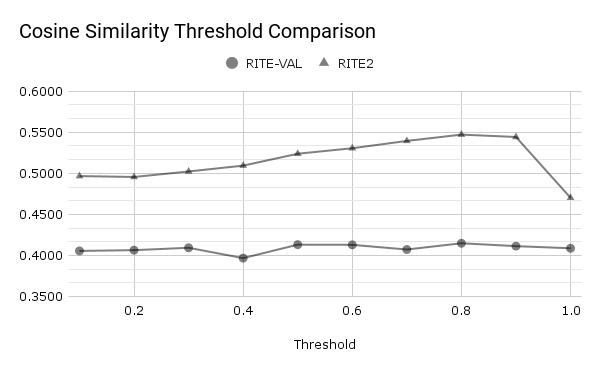
\includegraphics[width=15cm]{SimThresholdComp.png}
  \caption{Comparison of the Cosine Similarity Threshold of the Similarity-Based Word Sequence}
  \label{fig:threshold}
\end{figure}

\begin{table}[H]
  \centering
  \setlength{\extrarowheight}{-3pt}
  \caption{Comparison of the Cosine Similarity Threshold}
  \label{result:threshold_comparison}
  \begin{tabular}{|c|C{1.5cm}|C{1.5cm}|C{1.5cm}|C{1.5cm}|}
  \hline
  \multirow{2}{*}{Threshold} & \multicolumn{2}{c|}{RITE2} & \multicolumn{2}{c|}{RITE-VAL} \\ \cline{2-5}
   & \multicolumn{1}{c|}{Training} & \multicolumn{1}{c|}{Test} & \multicolumn{1}{c|}{Training} & \multicolumn{1}{c|}{Test} \\ \hline
  0.7 & 0.5395 & 0.3911 & 0.4072 & 0.3243 \\ \hline
  0.8 & \textbf{0.5472} & \textbf{0.3981} & \textbf{0.4133} & 0.3327 \\ \hline
  0.9 & 0.5443 & 0.3947 & 0.4113 & \textbf{0.3349} \\ \hline
  1.0 & 0.4702 & 0.3063 & 0.4087 & 0.2968 \\ \hline
  \end{tabular}
\end{table}

\paragraph{}
We want to know the performance of the similarity-based word sequence combines with machine learning features. We use an augmented RAD model to concatenate the machine learning features with the hidden states of similarity-based word sequence that encoded with a single RNN layer.

\paragraph{}
The results are shown in Table \ref{result:csa_nn}. Most of the performances are better than the neural network input by similarity-based word sequence only. This result proves that the machine learning features are beneficial to the systems.

\begin{table}[H]
  \centering
  \setlength{\extrarowheight}{-3pt}
  \caption{Comparison of the Features in the Neural Network}
  \label{result:csa_nn}
  \begin{tabular}{|l|C{1.5cm}|C{1.5cm}|C{1.5cm}|C{1.5cm}|}
  \hline
  \multicolumn{1}{|c|}{\multirow{2}{*}{Feature}} & \multicolumn{2}{c|}{RITE2} & \multicolumn{2}{c|}{RITE-VAL} \\ \cline{2-5}
  \multicolumn{1}{|c|}{} & \multicolumn{1}{c|}{Training} & \multicolumn{1}{c|}{Test} & \multicolumn{1}{c|}{Training} & \multicolumn{1}{c|}{Test} \\ \hline
  fastText Skip-Gram & 0.3801 & 0.2715 & 0.3882 & 0.2445 \\ \hline
  ft. SWS & \textbf{0.5415} & 0.4015 & 0.4062 & 0.3137 \\ \hline
  ft. SWS \& ML Features & 0.5407 & \textbf{0.4069} & \textbf{0.4283} & \textbf{0.3364} \\ \hline
  \end{tabular}
\end{table}

\paragraph{}
We compare the performance of the recurrent neural network whether to use the similarity-based word sequence and the machine learning features. We use CNLI as the training data. The results are shown in Table \ref{result:rnn_cnli}. We can see that the similarity-based word sequence and the machine learning features have huge improvements when using a ten thousand level dataset.

% ?? 補上 BERT + CNLI + SWS + MLFT 的實驗並填入 BERT + CNLI 的數據
% ?X?X 最後再來補的實驗:使用 Two-step pretraining on RNN
\begin{table}[H]
  \centering
  \setlength{\extrarowheight}{-3pt}
  \caption{Using CNLI as Training Data in the Recurrent Neural Network Experiments}
  \label{result:rnn_cnli}
  \begin{tabular}{|l|C{1.5cm}|C{1.5cm}|C{1.5cm}|C{1.5cm}|}
  \hline
  \multicolumn{1}{|c|}{\multirow{2}{*}{System}} & \multicolumn{2}{c|}{RITE2} & \multicolumn{2}{c|}{RITE-VAL} \\ \cline{2-5}
  \multicolumn{1}{|c|}{} & \multicolumn{1}{c|}{Training} & \multicolumn{1}{c|}{Test} & \multicolumn{1}{c|}{Training} & \multicolumn{1}{c|}{Test} \\ \hline
  RAD & 0.2849 & 0.2926 & 0.3314 & 0.2710 \\ \hline
  RAD + SWS + MLFT & \textbf{0.4847} & \textbf{0.4643} & \textbf{0.4601} & \textbf{0.3762} \\ \hline
  \end{tabular}
\end{table}

\paragraph{}
% 我們試著將 CSA 與 ML Features 這兩種方法與 BERT 模型做結合。與 CSA 結合的部份,我們先透過一層 RNN 進行 Encoding 然後與 BERT Hidden State 拼接在一起進行輸出,而 ML Features 的部份則是直接拼接並進行輸出,最後還有將三者做結合的實驗,並以 CNLI 做為 benchmark。其實驗結果如表,從 RITE-VAL 的角度來看,加入 CSA 與 ML Features 的做法並沒有帶來正面的提昇,而從 RITE2 的角度而言,效能的提昇也是相當微幅。可見 BERT 所能學習到的特徵表示是相當深入的。
We try to combine the BERT model with the similarity-based word sequence and the machine learning features to see how these features will impact the performance. We use the MNLI dataset and the CNLI-CT dataset as the benchmark.

\paragraph{}
In the combination of similarity-based word sequence, we first encode the similarity-based word sequence features with a recurrent neural network layer and concatenate them with BERT hidden states to output. In the machine learning features, we concatenate the features with BERT hidden states directly. Finally, we concatenate three of them for comparison.

\paragraph{}
The results are shown in Table \ref{tab:mnli_cnli_mlft_sws}. No matter the similarity-based word sequence, machine learning features, or the combination of both have no significant improvement to RITE. We can see that the feature representation that the BERT model can learn is quite in-depth.

% \paragraph{}
% We use the machine learning features and similarity-based word sequence in BERT. The first part uses MNLI as training data, and the second part uses two-step pre-training with MNLI and CNLI. The results are show in Table \ref{tab:mnli_cnli_mlft_sws}. We can see that these methods have bad influence to the system.

\begin{table}[H]
  \centering
  \setlength{\extrarowheight}{-3pt}
  \caption{Results of MNLI and CNLI with Machine Learning Features and Similarity-Based Word Sequence}
  \label{tab:mnli_cnli_mlft_sws}
  \begin{tabular}{|l|C{1.5cm}|C{1.5cm}|C{1.5cm}|C{1.5cm}|}
  \hline
  \multicolumn{1}{|c|}{\multirow{2}{*}{System}} & \multicolumn{2}{c|}{RITE2} & \multicolumn{2}{c|}{RITE-VAL} \\ \cline{2-5}
  \multicolumn{1}{|c|}{} & \multicolumn{1}{c|}{Training} & \multicolumn{1}{c|}{Test} & \multicolumn{1}{c|}{Training} & \multicolumn{1}{c|}{Test} \\ \hline
  MNLI & 0.6919 & 0.7107 & 0.5713 & 0.5561 \\ \hline
  MNLI \& MLFT & 0.6697 & 0.7032 & 0.5216 & 0.5301 \\ \hline
  MNLI \& SWS & 0.4459 & 0.3473 & 0.3275 & 0.2614 \\ \hline
  MNLI \& MLFT \& SWS & 0.5739 & 0.6077 & 0.4812 & 0.4414 \\ \hline \hline
  MNLI $\Rightarrow$ CNLI & 0.6952 & 0.6955 & 0.5811 & 0.5650 \\ \hline
  MNLI $\Rightarrow$ CNLI \& MLFT & 0.6444 & 0.6929 & 0.5375 & 0.5440 \\ \hline
  MNLI $\Rightarrow$ CNLI \& SWS & 0.4581 & 0.3911 & 0.3809 & 0.3204 \\ \hline
  MNLI $\Rightarrow$ CNLI \& MLFT \& SWS & 0.6004 & 0.6342 & 0.5071 & 0.4908 \\ \hline
  \end{tabular}
\end{table}

\subsection{Experiments with Generation-Based Data Expansion}
\paragraph{}
We use the pseudo training data as the training dataset to train BERT and fine-tune it with RITE. We also try to mix the pseudo dataset with CNLI and MNLI to see the performance. Rule-Based Pseudo-NLI is called RPNLI. GPT-2 Pseudo-NLI is called GPNLI. Half Pseudo-NLI is mixed with half of RPNLI and half of GPNLI, which is called HPNLI. All Pseudo-NLI is mixed with complete RPNLI and GPNLI, which is called APNLI.

\paragraph{}
The results are shown in Table \ref{result:pseudo_nli_bert}. We can see the performance of the rule-based pseudo dataset is better than the GPT-2 pseudo dataset. The performance of rule-based pseudo dataset mixed with CNLI is better than the performance of CNLI.

\paragraph{}
In RITE2, the performances of MNLI mixed with pseudo training data are better than CNLI mixed with pseudo training data, but not in RITE-VAL. Since RITE-VAL is more difficult than RITE2, we believe that the natural Chinese training data is necessary.

\begin{table}[H]
  \centering
  \setlength{\extrarowheight}{-3pt}
  \caption{Results of the BERT Trained with Pseudo-NLI and Fine-Tune with RITE}
  \label{result:pseudo_nli_bert}
  \begin{tabular}{|l|C{1.5cm}|C{1.5cm}|C{1.5cm}|C{1.5cm}|}
  \hline
  \multicolumn{1}{|c|}{\multirow{2}{*}{Dataset}} & \multicolumn{2}{c|}{RITE2} & \multicolumn{2}{c|}{RITE-VAL} \\ \cline{2-5}
  \multicolumn{1}{|c|}{} & \multicolumn{1}{c|}{Training} & \multicolumn{1}{c|}{Test} & \multicolumn{1}{c|}{Training} & \multicolumn{1}{c|}{Test} \\ \hline
  RPNLI & 0.6541 & \textbf{0.5777} & \textbf{0.5524} & 0.4257 \\ \hline
  GPNLI & 0.6283 & 0.5378 & 0.5156 & 0.4210 \\ \hline
  HPNLI & 0.6440 & 0.5462 & 0.5255 & 0.4276 \\ \hline
  APNLI & \textbf{0.6695} & 0.5659 & 0.5258 & \textbf{0.4440} \\ \hline \hline
  CNLI-CT & \textit{0.6848} & \textit{0.6426} & \textit{0.5915} & \textit{0.5146} \\ \hline
  CNLI-CT + RPNLI & 0.6908 & \textbf{0.6710} & 0.5992 & \textbf{0.5423} \\ \hline
  CNLI-CT + GPNLI & 0.6687 & 0.6409 & 0.5964 & 0.5364 \\ \hline
  CNLI-CT + HPNLI & 0.6881 & 0.6572 & 0.5858 & 0.5317 \\ \hline
  CNLI-CT + APNLI & \textbf{0.6940} & 0.6595 & \textbf{0.6114} & 0.5335 \\ \hline \hline
  MNLI & \textit{0.6919} & \textit{0.7107} & \textit{0.5713} & \textit{0.5561} \\ \hline
  MNLI   + RPNLI & 0.6796 & \textbf{0.6841} & 0.5576 & \textbf{0.5222} \\ \hline
  MNLI + GPNLI & 0.6818 & 0.6619 & 0.5603 & 0.4947 \\ \hline
  MNLI   + HPNLI & \textbf{0.6982} & 0.6574 & \textbf{0.5698} & 0.5191 \\ \hline
  MNLI   + APNLI & 0.6895 & 0.6639 & 0.5626 & 0.4925 \\ \hline
  \end{tabular}
\end{table}

\paragraph{}
% 我們比較了 MNLI 與 PNLI 使用兩步驟預訓練和混合資料集兩種方法
We compare the performance of two methods, two-step pre-training and dataset mixing, that using MNLI and PNLI. The results are shown in Table \ref{tab:cmp_mixed_2step}. We can see that the method of dataset mixing is better than two-step pre-training in this experiment.

\begin{table}[H]
  \centering
  \setlength{\extrarowheight}{-3pt}
  \caption{Comparison of Two-Step Pre-Training and Dataset Mixing}
  \label{tab:cmp_mixed_2step}
  \begin{tabular}{|l|C{1.5cm}|C{1.5cm}|C{1.5cm}|C{1.5cm}|}
  \hline
  \multicolumn{1}{|c|}{\multirow{2}{*}{System}} & \multicolumn{2}{c|}{RITE2} & \multicolumn{2}{c|}{RITE-VAL} \\ \cline{2-5}
  \multicolumn{1}{|c|}{} & \multicolumn{1}{c|}{Training} & \multicolumn{1}{c|}{Test} & \multicolumn{1}{c|}{Training} & \multicolumn{1}{c|}{Test} \\ \hline
  MNLI $\Rightarrow$ RPNLI & \textbf{0.6899} & \textbf{0.6364} & 0.5536 & \textbf{0.4836} \\ \hline
  MNLI $\Rightarrow$ GPNLI & 0.6404 & 0.6016 & 0.5092 & 0.4483 \\ \hline
  MNLI $\Rightarrow$ HPNLI & 0.6892 & 0.6293 & \textbf{0.5578} & 0.4817 \\ \hline
  MNLI $\Rightarrow$ APNLI & 0.6646 & 0.6158 & 0.5128 & 0.4652 \\ \hline \hline
  MNLI + RPNLI & 0.6796 & \textbf{0.6841} & 0.5576 & \textbf{0.5222} \\ \hline
  MNLI + GPNLI & 0.6818 & 0.6619 & 0.5603 & 0.4947 \\ \hline
  MNLI + HPNLI & \textbf{0.6982} & 0.6574 & \textbf{0.5698} & 0.5191 \\ \hline
  MNLI + APNLI & 0.6895 & 0.6639 & 0.5626 & 0.4925 \\ \hline
  \end{tabular}
\end{table}

\section{Conclusion} \label{section:conclusion}
\paragraph{}
% 文意蘊含系統在自然語言領域裡是相當核心的技術,藉由深度學習的方法,大幅降低了過去特徵工程的複雜性,而讓研究者可以更專注於在適當領域的文本探勘,將資源與成果較為豐富的語言轉移到相對弱勢的繁體中文上。
Textual entailment recognizing system is a quite core technology in natural language processing. The complexity of feature engineering is significantly reduced by deep learning and the researchers can focus more on the data mining of the proper domain. And with the help of the cross-lingual resources, the language with rich resources can apply the result on the Traditional Chinese which is relatively weak in resources.

\paragraph{}
% 本論文主要提出三種系統,第一種是使用 Sentence-based features 的機器學習,第二種是綜合了 Sentence-based features, Word-based sequence features 與 WGA 三種特徵的 Neural Network,第三種是使用了 Cross-lingual Training 的 Transformers BERT。其中使用了 Cross-lingual Training 的 Transformers BERT 讓我們將 RITE 資料集的實驗推向深度學習的領域且實現了相當卓越的效能。
In this thesis, the best of our systems is the transformers BERT using cross-lingual training. This system lets us push the experiments of RITE datasets to the field of deep learning and achieved quite excellent performance.

\paragraph{}
% 在資料集改善的方面,除了 Reversed Labels 與資料集混合以外,我們也提出了使用 GPT-2 產生虛擬訓練資料的方法,透過實驗證實了這個方法有一定程度的效果,我們認為這個方法也相當具有潛力。未來若是有更強大的運算效能可以將這個實驗套用到 GPT-2-LARGE 或 GPT3 上可能會有更好的結果。
In the experiments of training data expansion, in addition to reversed labels and mixing datasets, the pseudo training data generated by rule-based and GPT-2 is proposed. We proved this method is effective. We think this method is quite potential. In the future, with more powerful computing performance, the GPT-2-LARGE or GPT-3 may be applied to the experiments and may get better performance.

\paragraph{}
% 核心模組皆為開源系統,本論文的實驗都具有高度的可重製性。我們希望這樣的研究方向與經歷可以提供給其他資源也同樣相對匱乏的語言的研究者一個參考。
Our core modules are open-source systems and our experiments are highly reproducible. We hope this research direction and experience may provide a reference for other research in the language which is also relatively low resources.

\end{spacing}

\addcontentsline{toc}{section}{References}
\bibliography{main}
\bibliographystyle{unsrtnat}
% \printbibliography

\begin{spacing}{1.77}
\phantomsection
\addcontentsline{toc}{section}{Appendix}
\section*{Appendix}

% ?? 可能要使用不同的 numbering

\paragraph{}
Table \ref{result:bert-rite-val-dev} shows the detailed performance of the RITE-VAL training set. Table \ref{result:bert-rite-val-test} shows the detailed performance of the RITE-VAL test set. Table \ref{result:bert-rite2-dev} shows the detailed performance of the RITE2 training set. Table \ref{result:bert-rite2-test} shows the detailed performance of the RITE2 test set.

\paragraph{}
These detailed results show the F1-score of labels of BFCI task respectively. We can see that the F1-score of C and I is much lower than the F1-score of B and F. We believe that the patterns of C and I are more difficult to find. Especially the sample space of I is extremely large. The entailment relation between almost any two sentences in the real world is I.

\begin{table}[H]
  \centering
  \setlength{\extrarowheight}{-3pt}
  \caption{The Detailed Performance of the Different Systems in the RITE-VAL Training Set}
  \label{result:bert-rite-val-dev}
  \begin{tabular}{|l|C{1.75cm}|C{1.75cm}|C{1.75cm}|C{1.75cm}|C{1.75cm}|}
  \hline
  \multicolumn{6}{|c|}{RITE-VAL Training} \\ \hline
  \multicolumn{1}{|c|}{System} & \multicolumn{1}{c|}{B-F1} & \multicolumn{1}{c|}{F-F1} & \multicolumn{1}{c|}{C-F1} & \multicolumn{1}{c|}{I-F1} & \multicolumn{1}{c|}{Micro F1} \\ \hline
  CNLI-CT-Only & 0.7024 & 0.5022 & 0.4863 & 0.2157 & 0.4766 \\ \hline
  CNLI-CT & 0.7384 & 0.6754 & \textbf{0.6224} & 0.3299 & \textbf{0.5915} \\ \hline
  CNLI-CS & 0.6881 & 0.6424 & 0.5893 & 0.3238 & 0.5609 \\ \hline
  OCNLI-CT & 0.6870 & 0.6667 & 0.4948 & 0.2778 & 0.5316 \\ \hline \hline
  MNLI & 0.7478 & 0.6689 & 0.5567 & 0.3119 & 0.5713 \\ \hline
  MNLI $\Rightarrow$ CNLI-CT & \textbf{0.7522} & \textbf{0.6839} & 0.5895 & 0.2991 & 0.5811 \\ \hline
  MNLI + CNLI-CT & 0.7505 & 0.6537 & 0.5866 & \textbf{0.3670} & 0.5895 \\ \hline
  \end{tabular}
\end{table}

\begin{table}[H]
  \centering
  \setlength{\extrarowheight}{-3pt}
  \caption{The Detailed Performance of the Different Systems in the RITE-VAL Test Set}
  \label{result:bert-rite-val-test}
  \begin{tabular}{|l|C{1.75cm}|C{1.75cm}|C{1.75cm}|C{1.75cm}|C{1.75cm}|}
  \hline
  \multicolumn{6}{|c|}{RITE-VAL Test} \\ \hline
  \multicolumn{1}{|c|}{System} & \multicolumn{1}{c|}{B-F1} & \multicolumn{1}{c|}{F-F1} & \multicolumn{1}{c|}{C-F1} & \multicolumn{1}{c|}{I-F1} & \multicolumn{1}{c|}{Macro F1} \\ \hline
  CNLI-CT-Only & 0.6110 & 0.5506 & 0.5219 & 0.3135 & 0.4993 \\ \hline
  CNLI-CT & 0.6084 & 0.6172 & 0.5764 & 0.2565 & 0.5146 \\ \hline
  CNLI-CS & 0.5316 & 0.6077 & 0.5579 & 0.2936 & 0.4977 \\ \hline
  OCNLI-CT & 0.5608 & 0.6091 & 0.5517 & 0.3153 & 0.5092 \\ \hline \hline
  MNLI & 0.6137 & 0.6291 & 0.6122 & 0.3696 & 0.5561 \\ \hline
  MNLI $\Rightarrow$ CNLI-CT & 0.6291 & \textbf{0.6365} & \textbf{0.6163} & \textbf{0.3780} & \textbf{0.5650} \\ \hline
  MNLI + CNLI-CT & \textbf{0.6326} & 0.6268 & 0.6042 & 0.3731 & 0.5592 \\ \hline
  \end{tabular}
\end{table}

\begin{table}[H]
  \centering
  \setlength{\extrarowheight}{-3pt}
  \caption{The Detailed Performance of the Different Systems in the RITE2 Training Set}
  \label{result:bert-rite2-dev}
  \begin{tabular}{|l|C{1.75cm}|C{1.75cm}|C{1.75cm}|C{1.75cm}|C{1.75cm}|}
  \hline
  \multicolumn{6}{|c|}{RITE2 Training} \\ \hline
  \multicolumn{1}{|c|}{System} & \multicolumn{1}{c|}{B-F1} & \multicolumn{1}{c|}{F-F1} & \multicolumn{1}{c|}{C-F1} & \multicolumn{1}{c|}{I-F1} & \multicolumn{1}{c|}{Micro F1} \\ \hline
  CNLI-CT-Only & 0.5443 & 0.7003 & 0.4158 & 0.4902 & 0.5377 \\ \hline
  CNLI-CT & 0.6827 & 0.8444 & 0.5493 & 0.6627 & 0.6848 \\ \hline
  CNLI-CS & 0.6718 & 0.8408 & 0.5167 & 0.6605 & 0.6724 \\ \hline
  OCNLI-CT & 0.6416 & 0.8406 & 0.5209 & 0.6810 & 0.6710 \\ \hline \hline
  MNLI & 0.6867 & \textbf{0.8640} & 0.5247 & \textbf{0.6920} & 0.6919 \\ \hline
  MNLI $\Rightarrow$ CNLI-CT & 0.6906 & 0.8551 & \textbf{0.5520} & 0.6830 & \textbf{0.6952} \\ \hline
  MNLI + CNLI-CT & \textbf{0.6962} & 0.8455 & 0.5322 & 0.6779 & 0.6880 \\ \hline
  \end{tabular}
\end{table}

% ?? 交換倒數兩個系統
\begin{table}[H]
  \centering
  \setlength{\extrarowheight}{-3pt}
  \caption{The Individual F1-Scores of BFCI Classes on the RITE2 Test Set}
  \label{result:bert-rite2-test}
  \begin{tabular}{|l|C{1.75cm}|C{1.75cm}|C{1.75cm}|C{1.75cm}|C{1.75cm}|}
  \hline
  \multicolumn{6}{|c|}{RITE2 Test} \\ \hline
  \multicolumn{1}{|c|}{System} & \multicolumn{1}{c|}{B-F1} & \multicolumn{1}{c|}{F-F1} & \multicolumn{1}{c|}{C-F1} & \multicolumn{1}{c|}{I-F1} & \multicolumn{1}{c|}{Macro F1} \\ \hline
  CNLI-CT-Only & 0.6797 & 0.6667 & 0.5035 & 0.5303 & 0.5950 \\ \hline
  CNLI-CT & 0.7140 & 0.7393 & 0.5315 & 0.5856 & 0.6426 \\ \hline
  CNLI-CS & 0.6796 & 0.7336 & 0.4811 & 0.6228 & 0.6293 \\ \hline
  OCNLI-CT & 0.6488 & 0.7120 & 0.4000 & 0.5928 & 0.5884 \\ \hline \hline
  MNLI & \textbf{0.7834} & 0.7881 & \textbf{0.5757} & \textbf{0.6955} & \textbf{0.7107} \\ \hline
  MNLI $\Rightarrow$ CNLI-CT & 0.7689 & 0.7748 & 0.5662 & 0.6721 & 0.6955 \\ \hline
  MNLI + CNLI-CT & 0.7731 & \textbf{0.7936} & 0.5604 & 0.6875 & 0.7036 \\ \hline
  \end{tabular}
\end{table}
\end{spacing}

\end{CJK*}
\end{document}
